\chapter{Bonus. Clasificación de Dígitos}

Clasificación de Dígitos. Considerar el conjunto de datos de dígitos
manuscritos, y seleccionar las muestras de los dígitos 4 y 8. 
Extraer las características de intensidad promedio y simetría en la
manera que se indicó en el ejercicio 3 de la práctica anterior.

\section{Planteamiento del problema de clasificación binaria asociado}

\textbf{Debe considerar el conjunto de entrenamiento como datos de entrada para aprender
la función $g$.}

El siguiente conjunto $\{\mathcal{X}, \mathcal{Y}, \mathcal{D}, f: \mathcal{X} \rightarrow \mathcal{Y}, \mathcal{A}_i, \mathcal{H}, g\}$
define 4 problemas de clasificación binaria con $i=1,2,3,4$ siendo los elementos:

\begin{itemize}
  \item $\mathcal{X} = \{1\} \times \mathbb{R}^2$
  \item $\mathcal{Y} = \{-1, 1\}$ donde $-1$ representa el dígito $4$ y $1$ el $8$.
  \item $\mathcal{D} = \{(x_n, y_n): n = 1,\dots N \} \subset \mathcal{X} \times \mathcal{Y}$
es el conjunto de $N$ datos de entrenamiento dentro del espacio de entrada con su correspondiente
salida (problema de clasificación binaria, aprendizaje supervisado).
  \item $f : \mathcal{X} \rightarrow \mathcal{Y}$ función objetivo, completamente desconocida que
aproximaremos a partir de los datos de entrenamiento.
  \item $\mathcal{H} = \{h \in \mathbb{R}^3 \rightarrow \mathbb{R} : h(x) = \text{sign}(w^Tx), w \in \mathbb{R}^3 \}$ : 
conjunto de hipótesis a partir del cual estimaremos $g \in \mathcal{H}$ suponiendo distribución de probabilidad
$\mathcal{P}$ en $\mathcal{X} \times \mathcal{Y}$ de acuerdo a la que se obtiene las $N$ instancias de $\mathcal{D}$ 
de forma independientemente e idénticamente distribuida.
  \item $\mathcal{A}_i$: algoritmo de aprendizaje
    \subitem $\mathcal{A}_1$: Algoritmo de la Pseudoinversa para Regresión Lineal
    \subitem $\mathcal{A}_2$: Algoritmo de Aprendizaje del Perceptrón (PLA)
    \subitem $\mathcal{A}_3$: Algoritmo SGD para Regresión Lineal (RL)
    \subitem $\mathcal{A}_4$: Algoritmo PLA-POCKET
  \item $g \in \mathcal{H}$: función del conjunto de hipótesis que usamos para aproximar $f$
  \item $\mathcal{L}_i$: función de pérdida (usada por $\mathcal{A}$ para aproximar g)
    \subitem $\mathcal{L}_1$: Error cuadrático medio
    \subitem $\mathcal{L}_2 = \mathcal{L}_4$ : Error de clasificación
    \subitem $\mathcal{L}_3$ : Error de entropía cruzada (véase apartado Reg. Log.)
\end{itemize}

\section{Comparación de los modelos lineales estudiados}

\textbf{Compárense los modelos de regresión lineal, PLA, RL y PLA-Pocket.}

\subsection{Generar gráficos con la función estimada sobre los datos de entrenamiento y test}

\begin{figure}[H]
    \caption{Regresión Lineal\medskip}
    \begin{minipage}[b]{.5\linewidth}
      \centering
      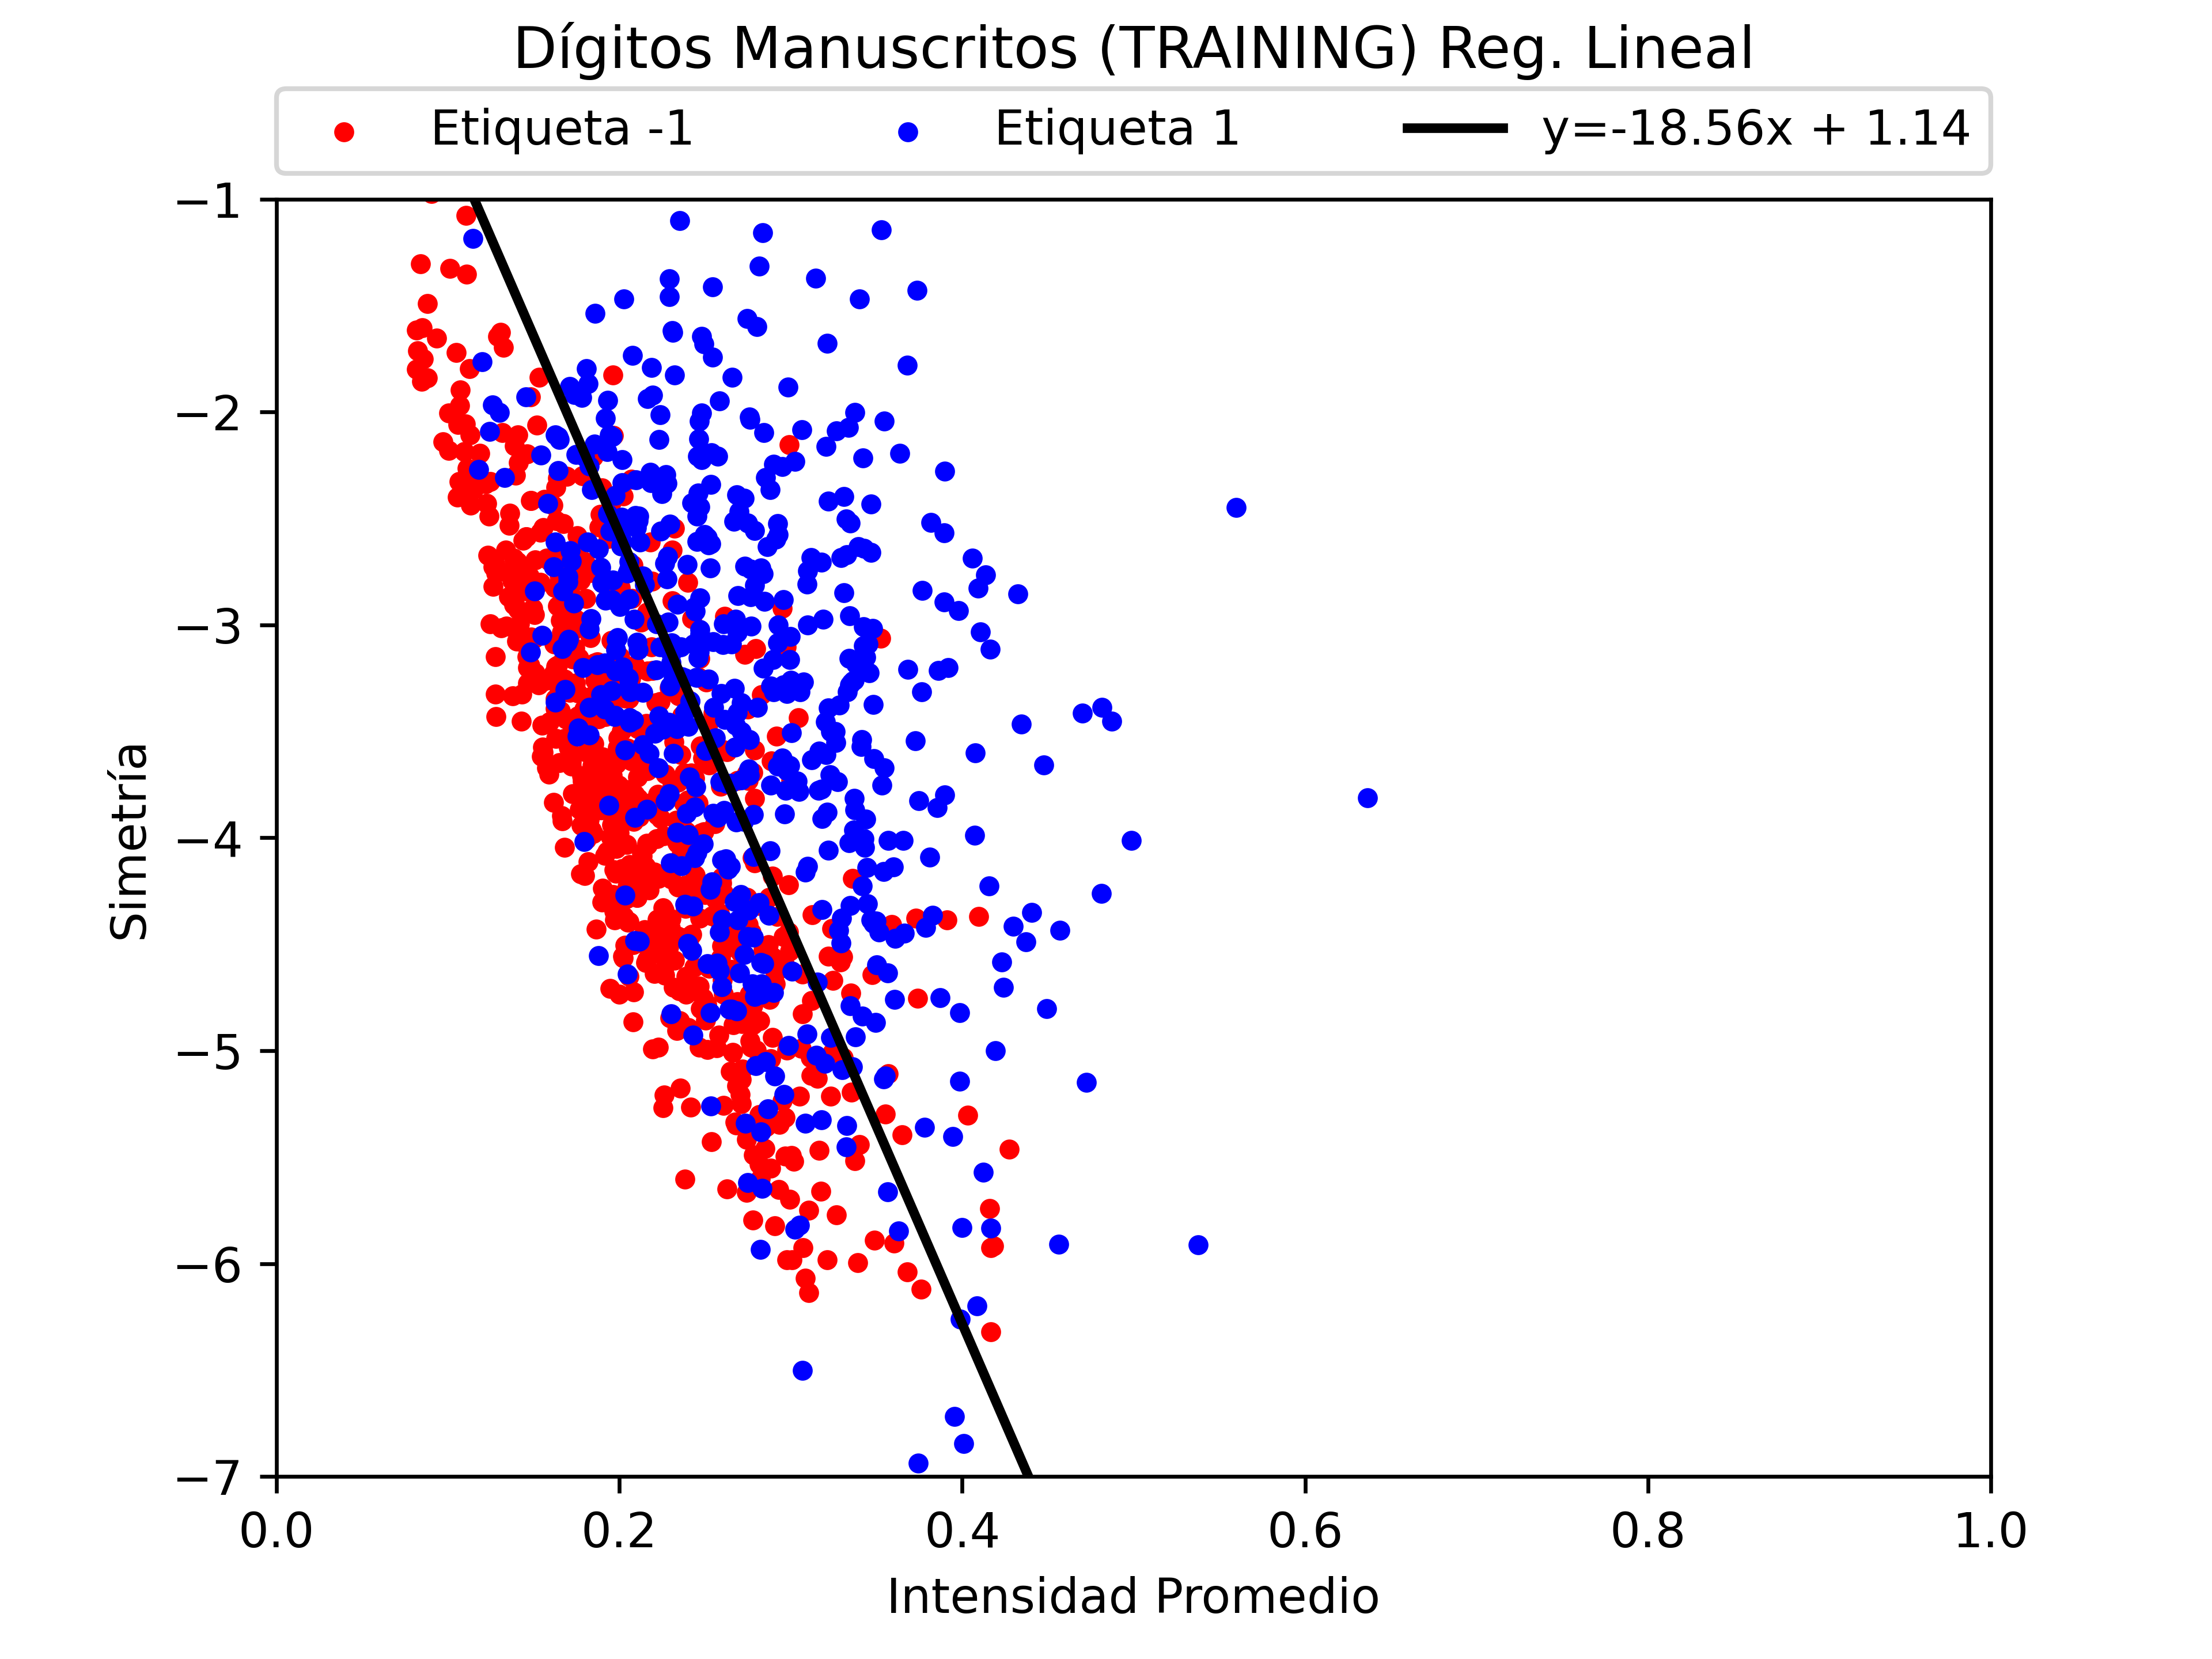
\includegraphics[width=0.9\textwidth]{Figure_15}
      \subcaption{Datos de entrenamiento} \label{subfig-5:dummy62}
    \end{minipage}
    \hfill \hfill
    \begin{minipage}[b]{.5\linewidth}
      \centering
      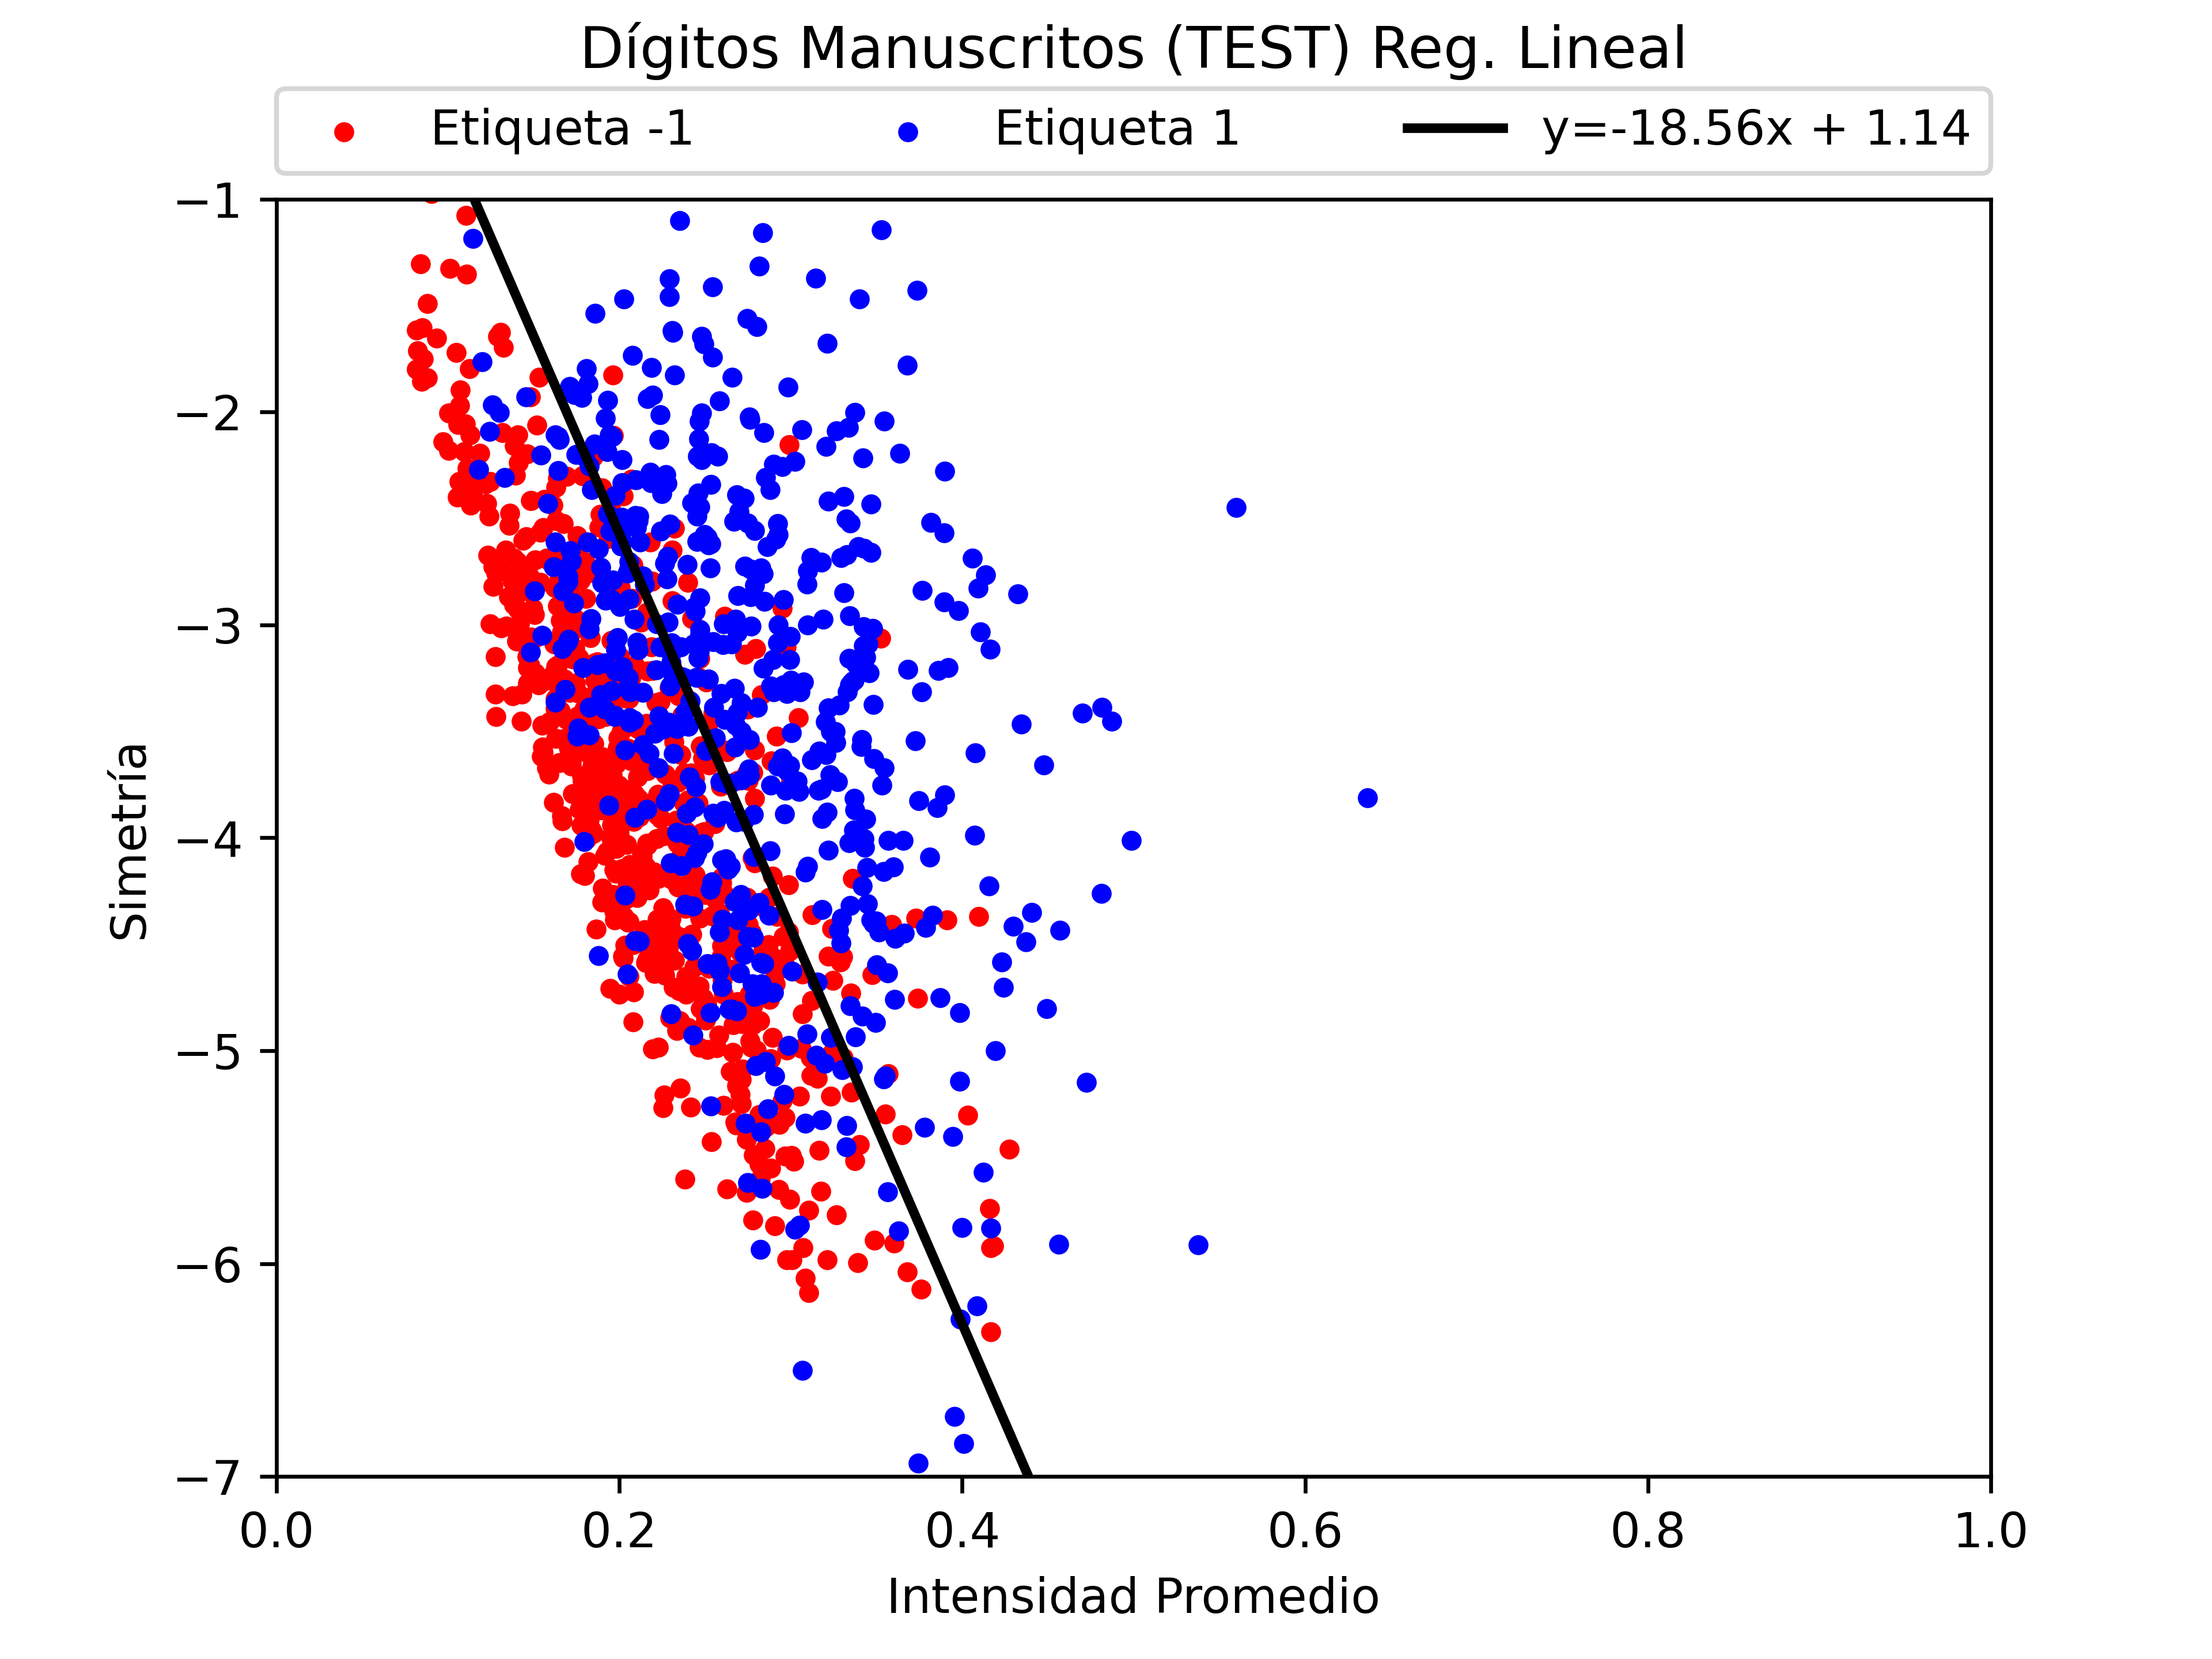
\includegraphics[width=0.9\textwidth]{Figure_16}
      \subcaption{Datos de test}
    \end{minipage}
    \label{fig:dummy62}
\end{figure}

\begin{figure}[H]
    \caption{PLA - Algoritmo de aprendizaje del perceptrón\medskip}
    \begin{minipage}[b]{.5\linewidth}
      \centering
      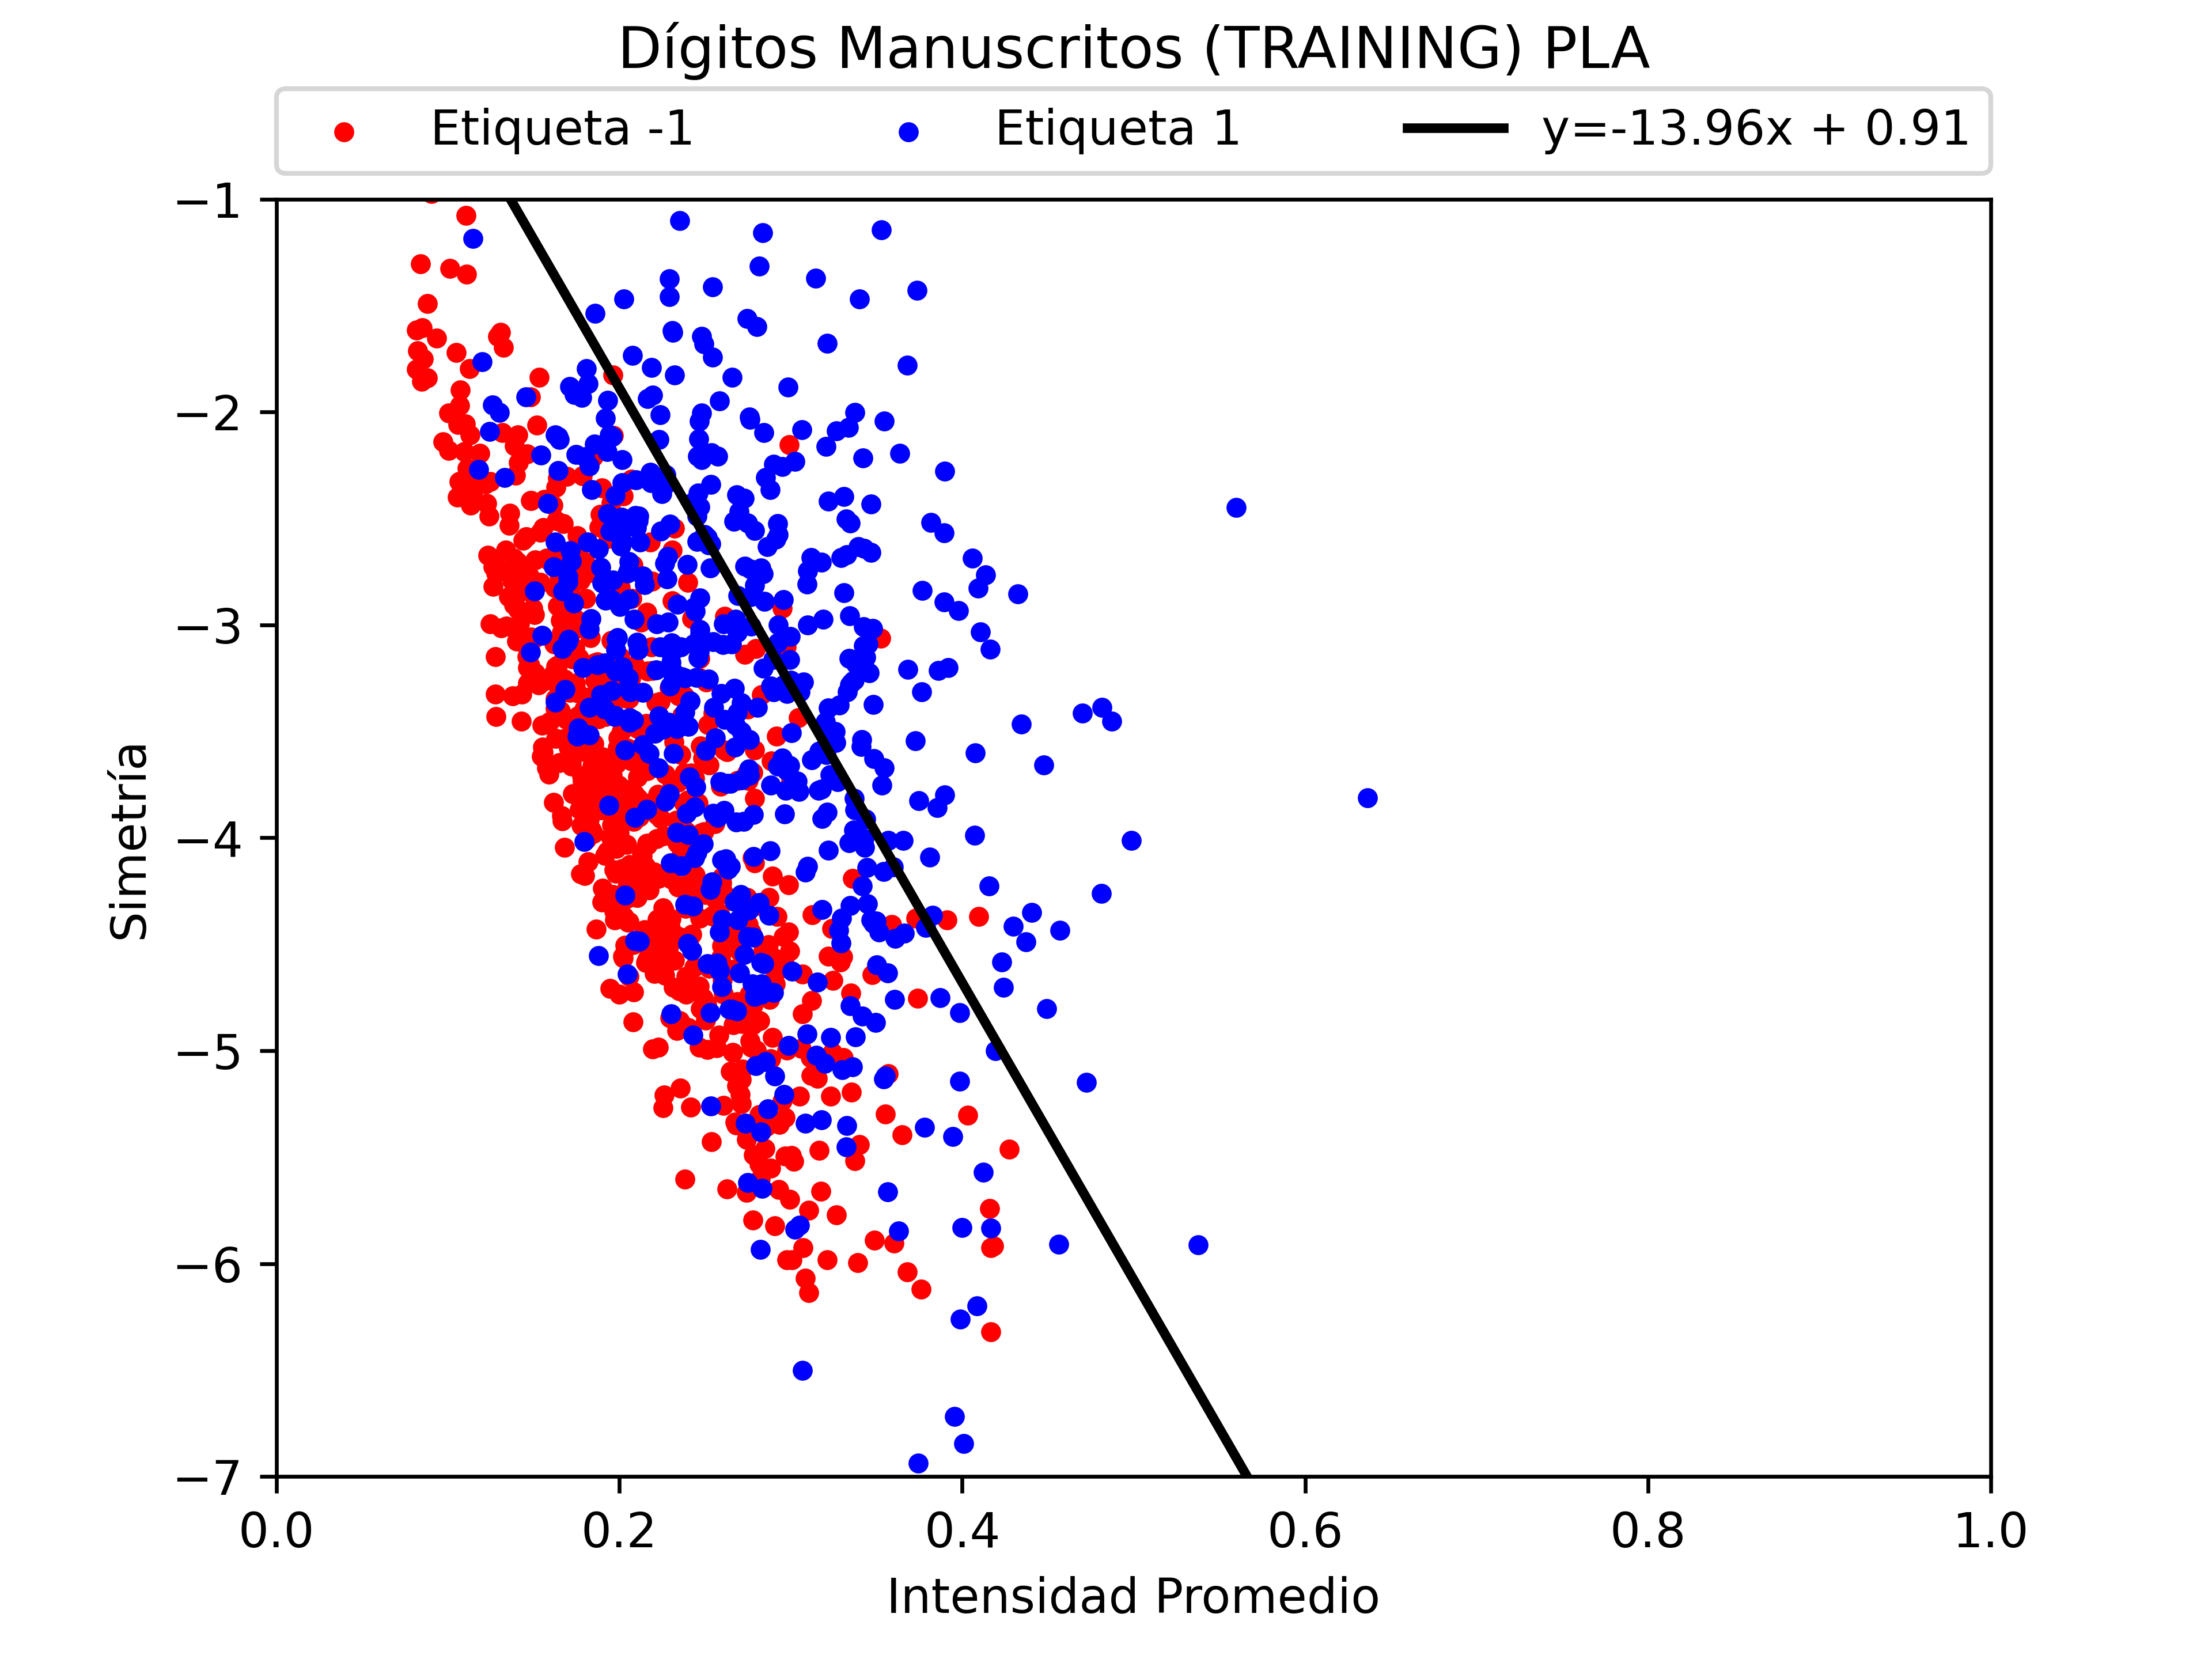
\includegraphics[width=0.9\textwidth]{Figure_17}
      \subcaption{Datos de entrenamiento} \label{subfig-5:dummy63}
    \end{minipage}
    \hfill \hfill
    \begin{minipage}[b]{.5\linewidth}
      \centering
      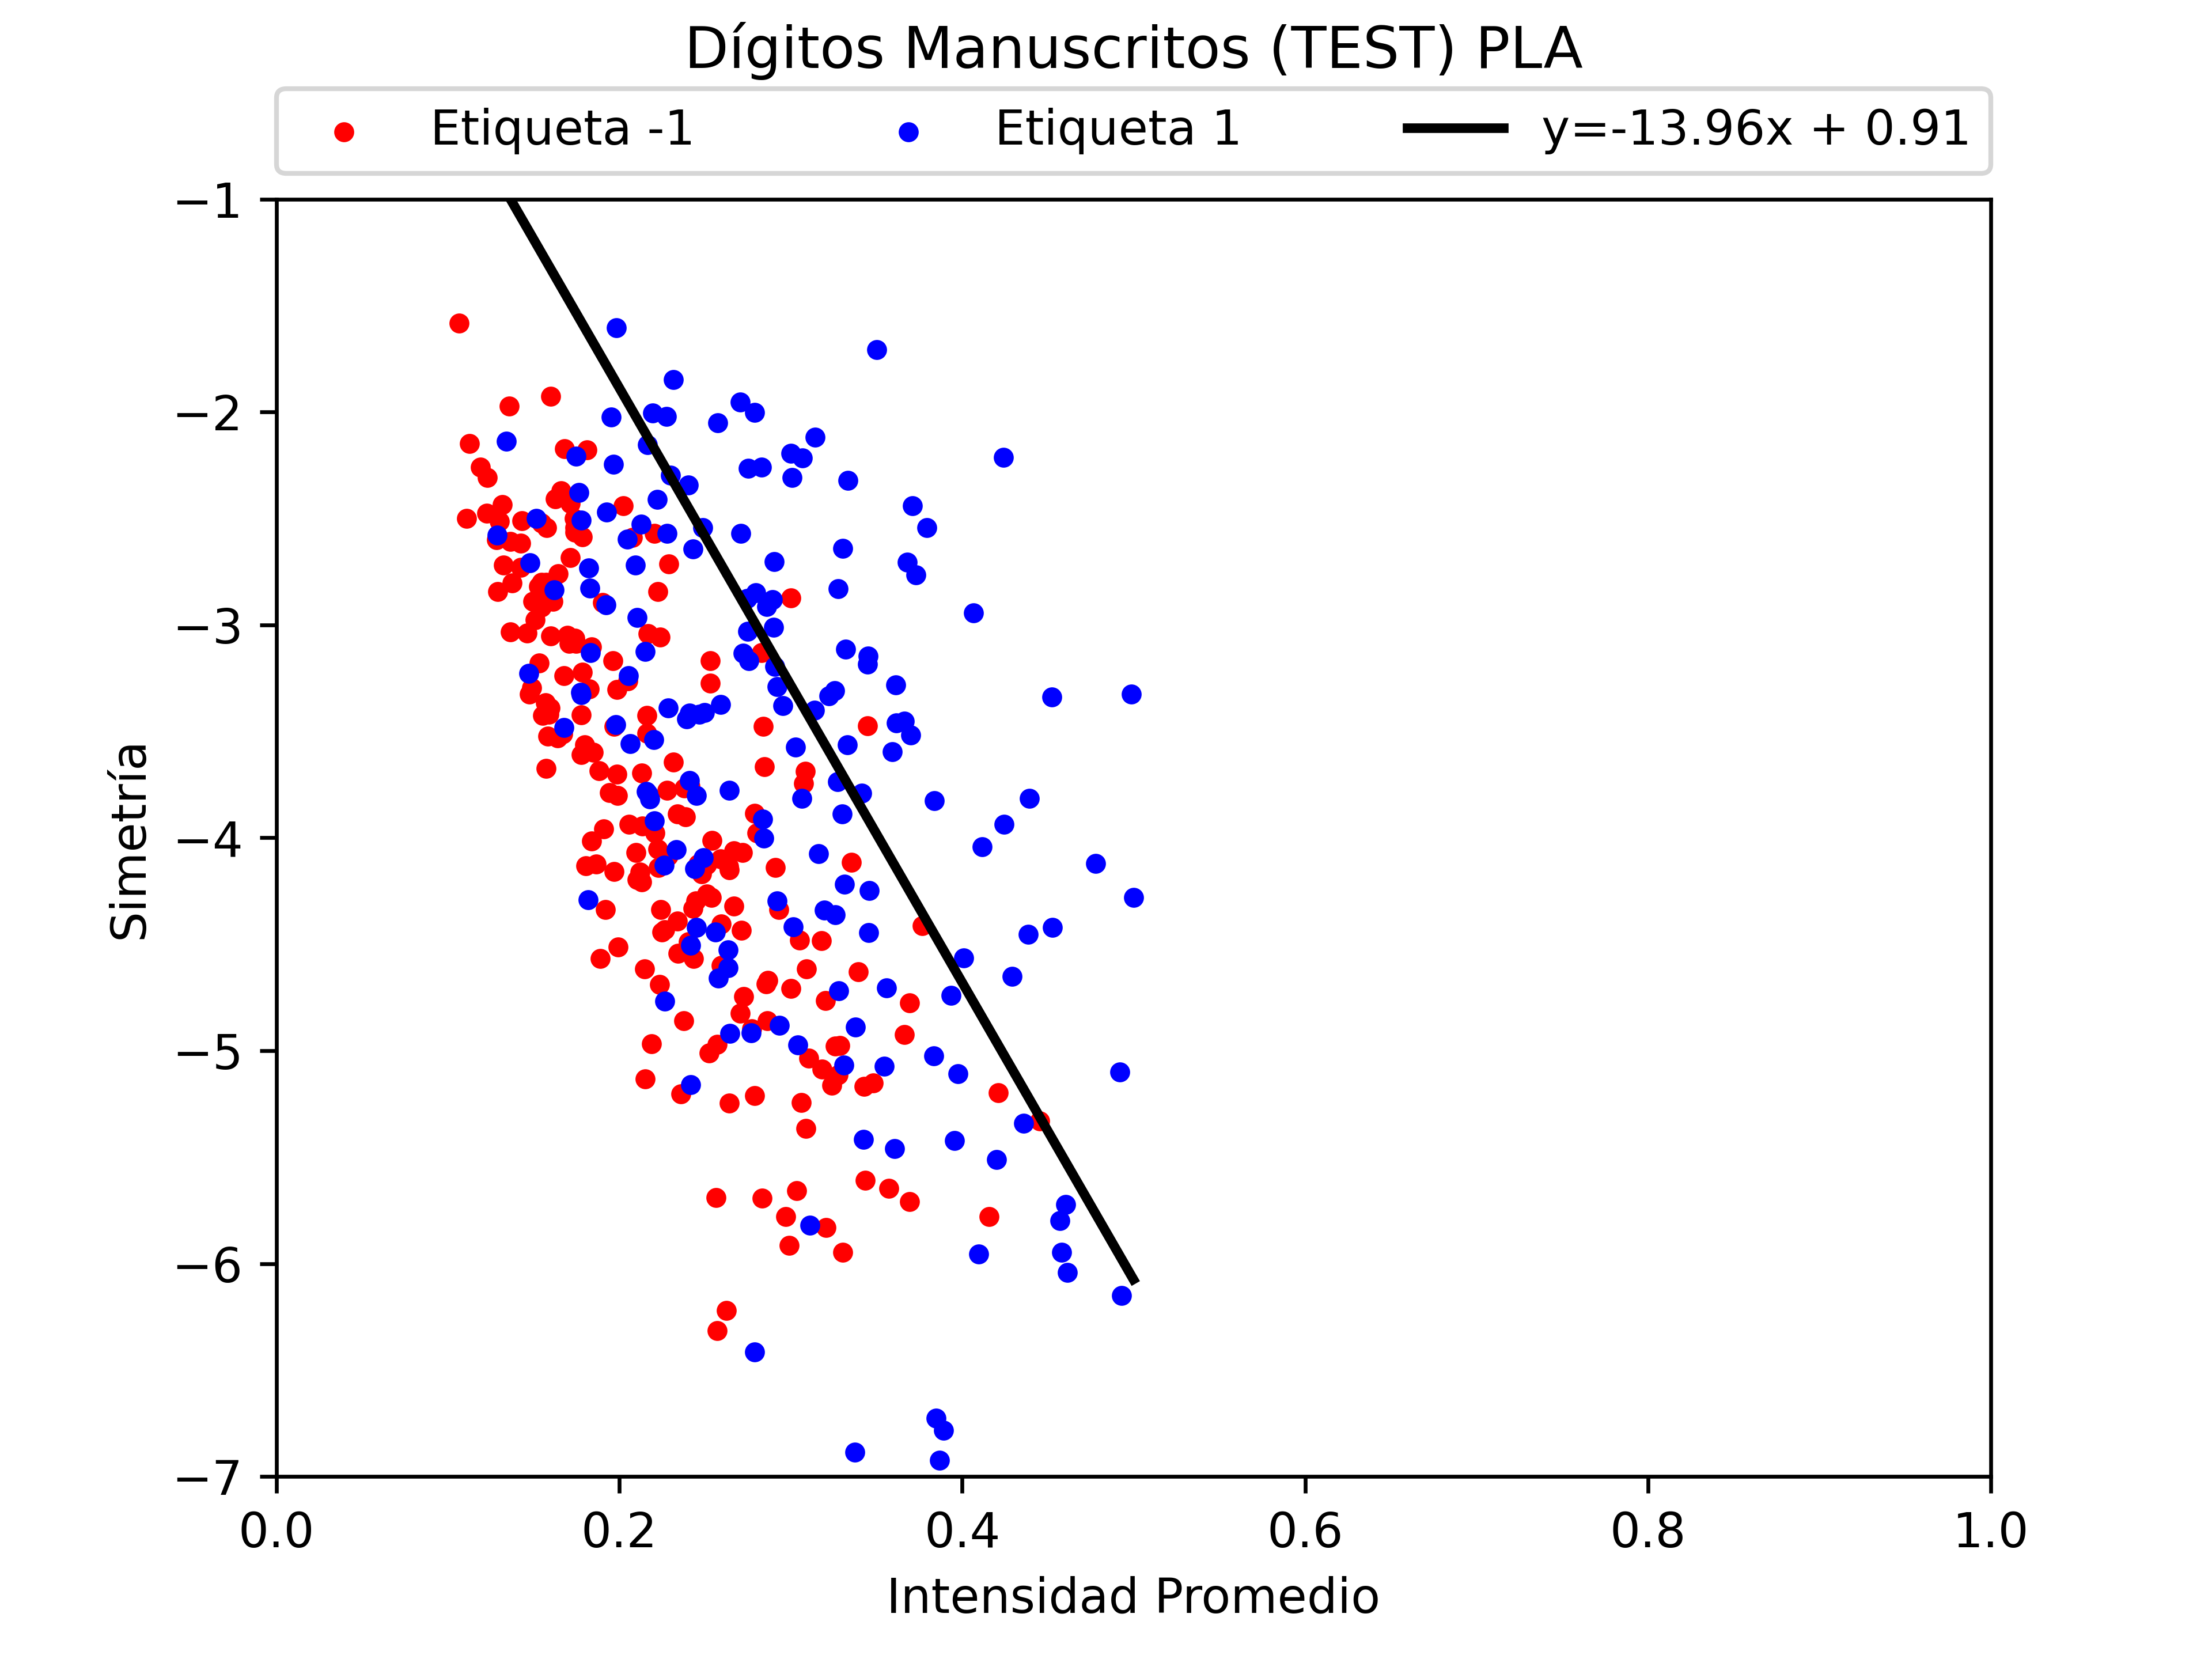
\includegraphics[width=0.9\textwidth]{Figure_18}
      \subcaption{Datos de test}
    \end{minipage}
    \label{fig:dummy63}
\end{figure}

\begin{figure}[H]
    \caption{RL - Regresión Logística para clasificación lineal\medskip}
    \begin{minipage}[b]{.5\linewidth}
      \centering
      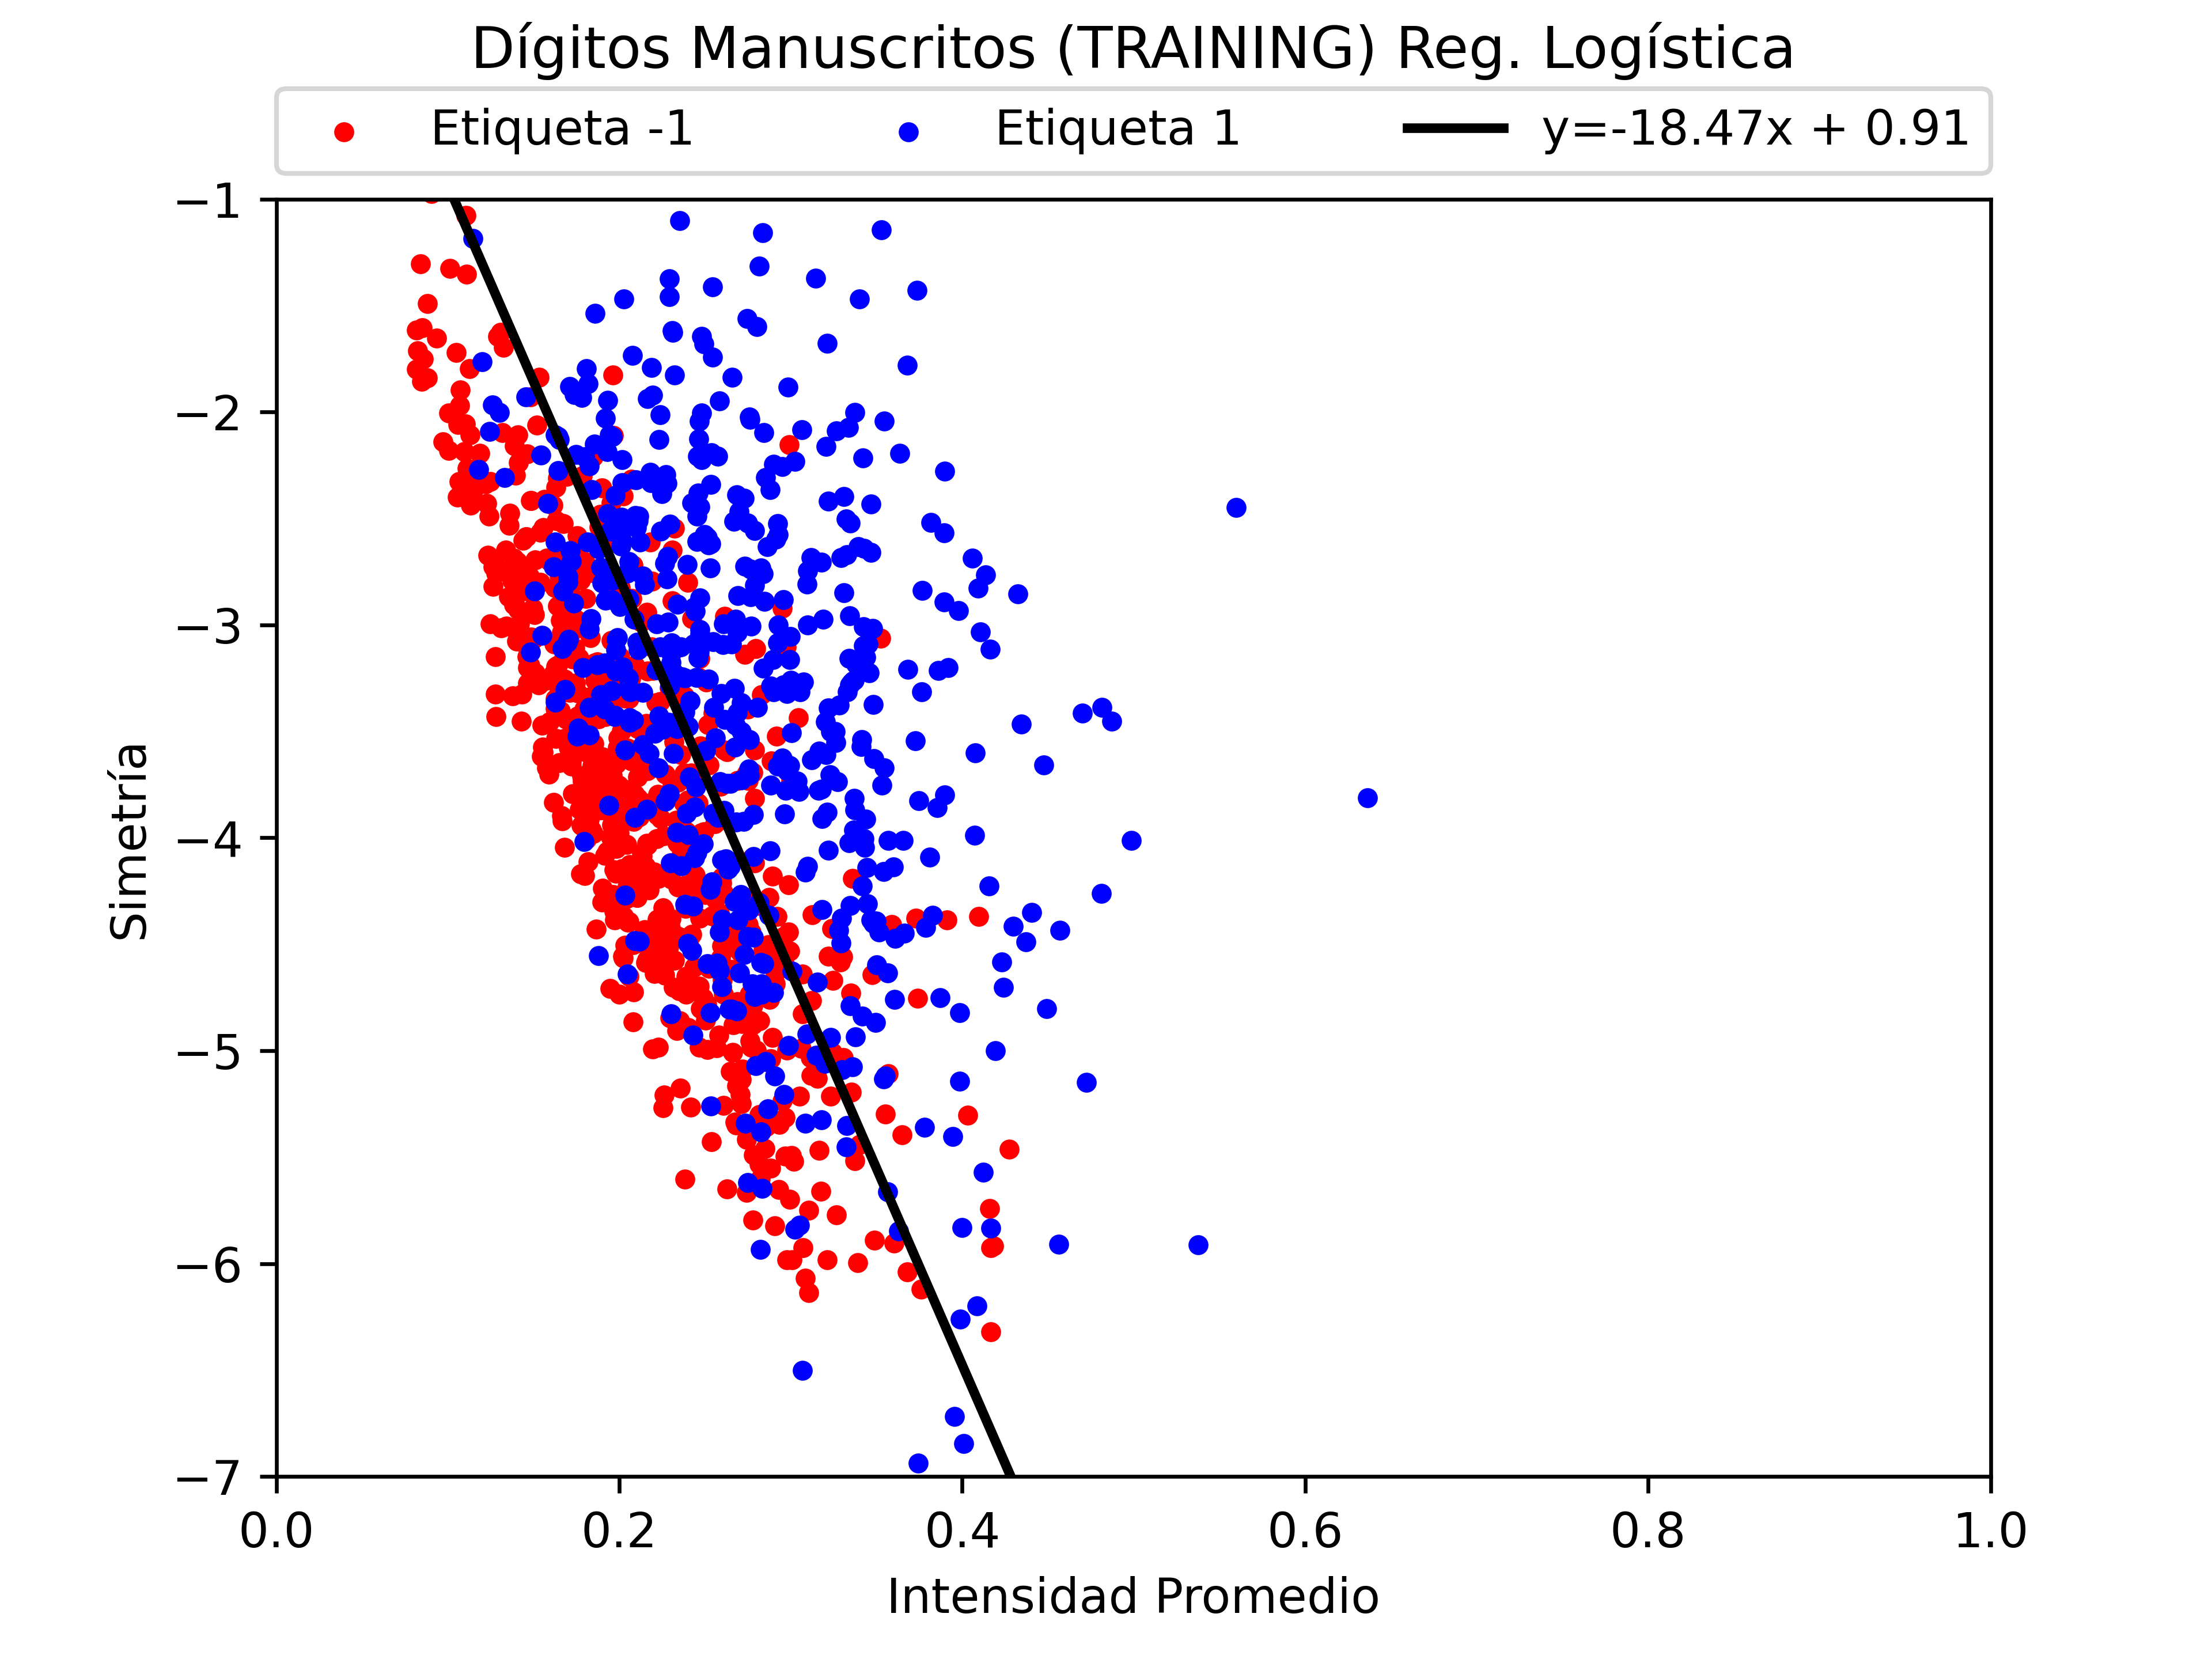
\includegraphics[width=0.9\textwidth]{Figure_19}
      \subcaption{Datos de entrenamiento} \label{subfig-5:dummy64}
    \end{minipage}
    \hfill \hfill
    \begin{minipage}[b]{.5\linewidth}
      \centering
      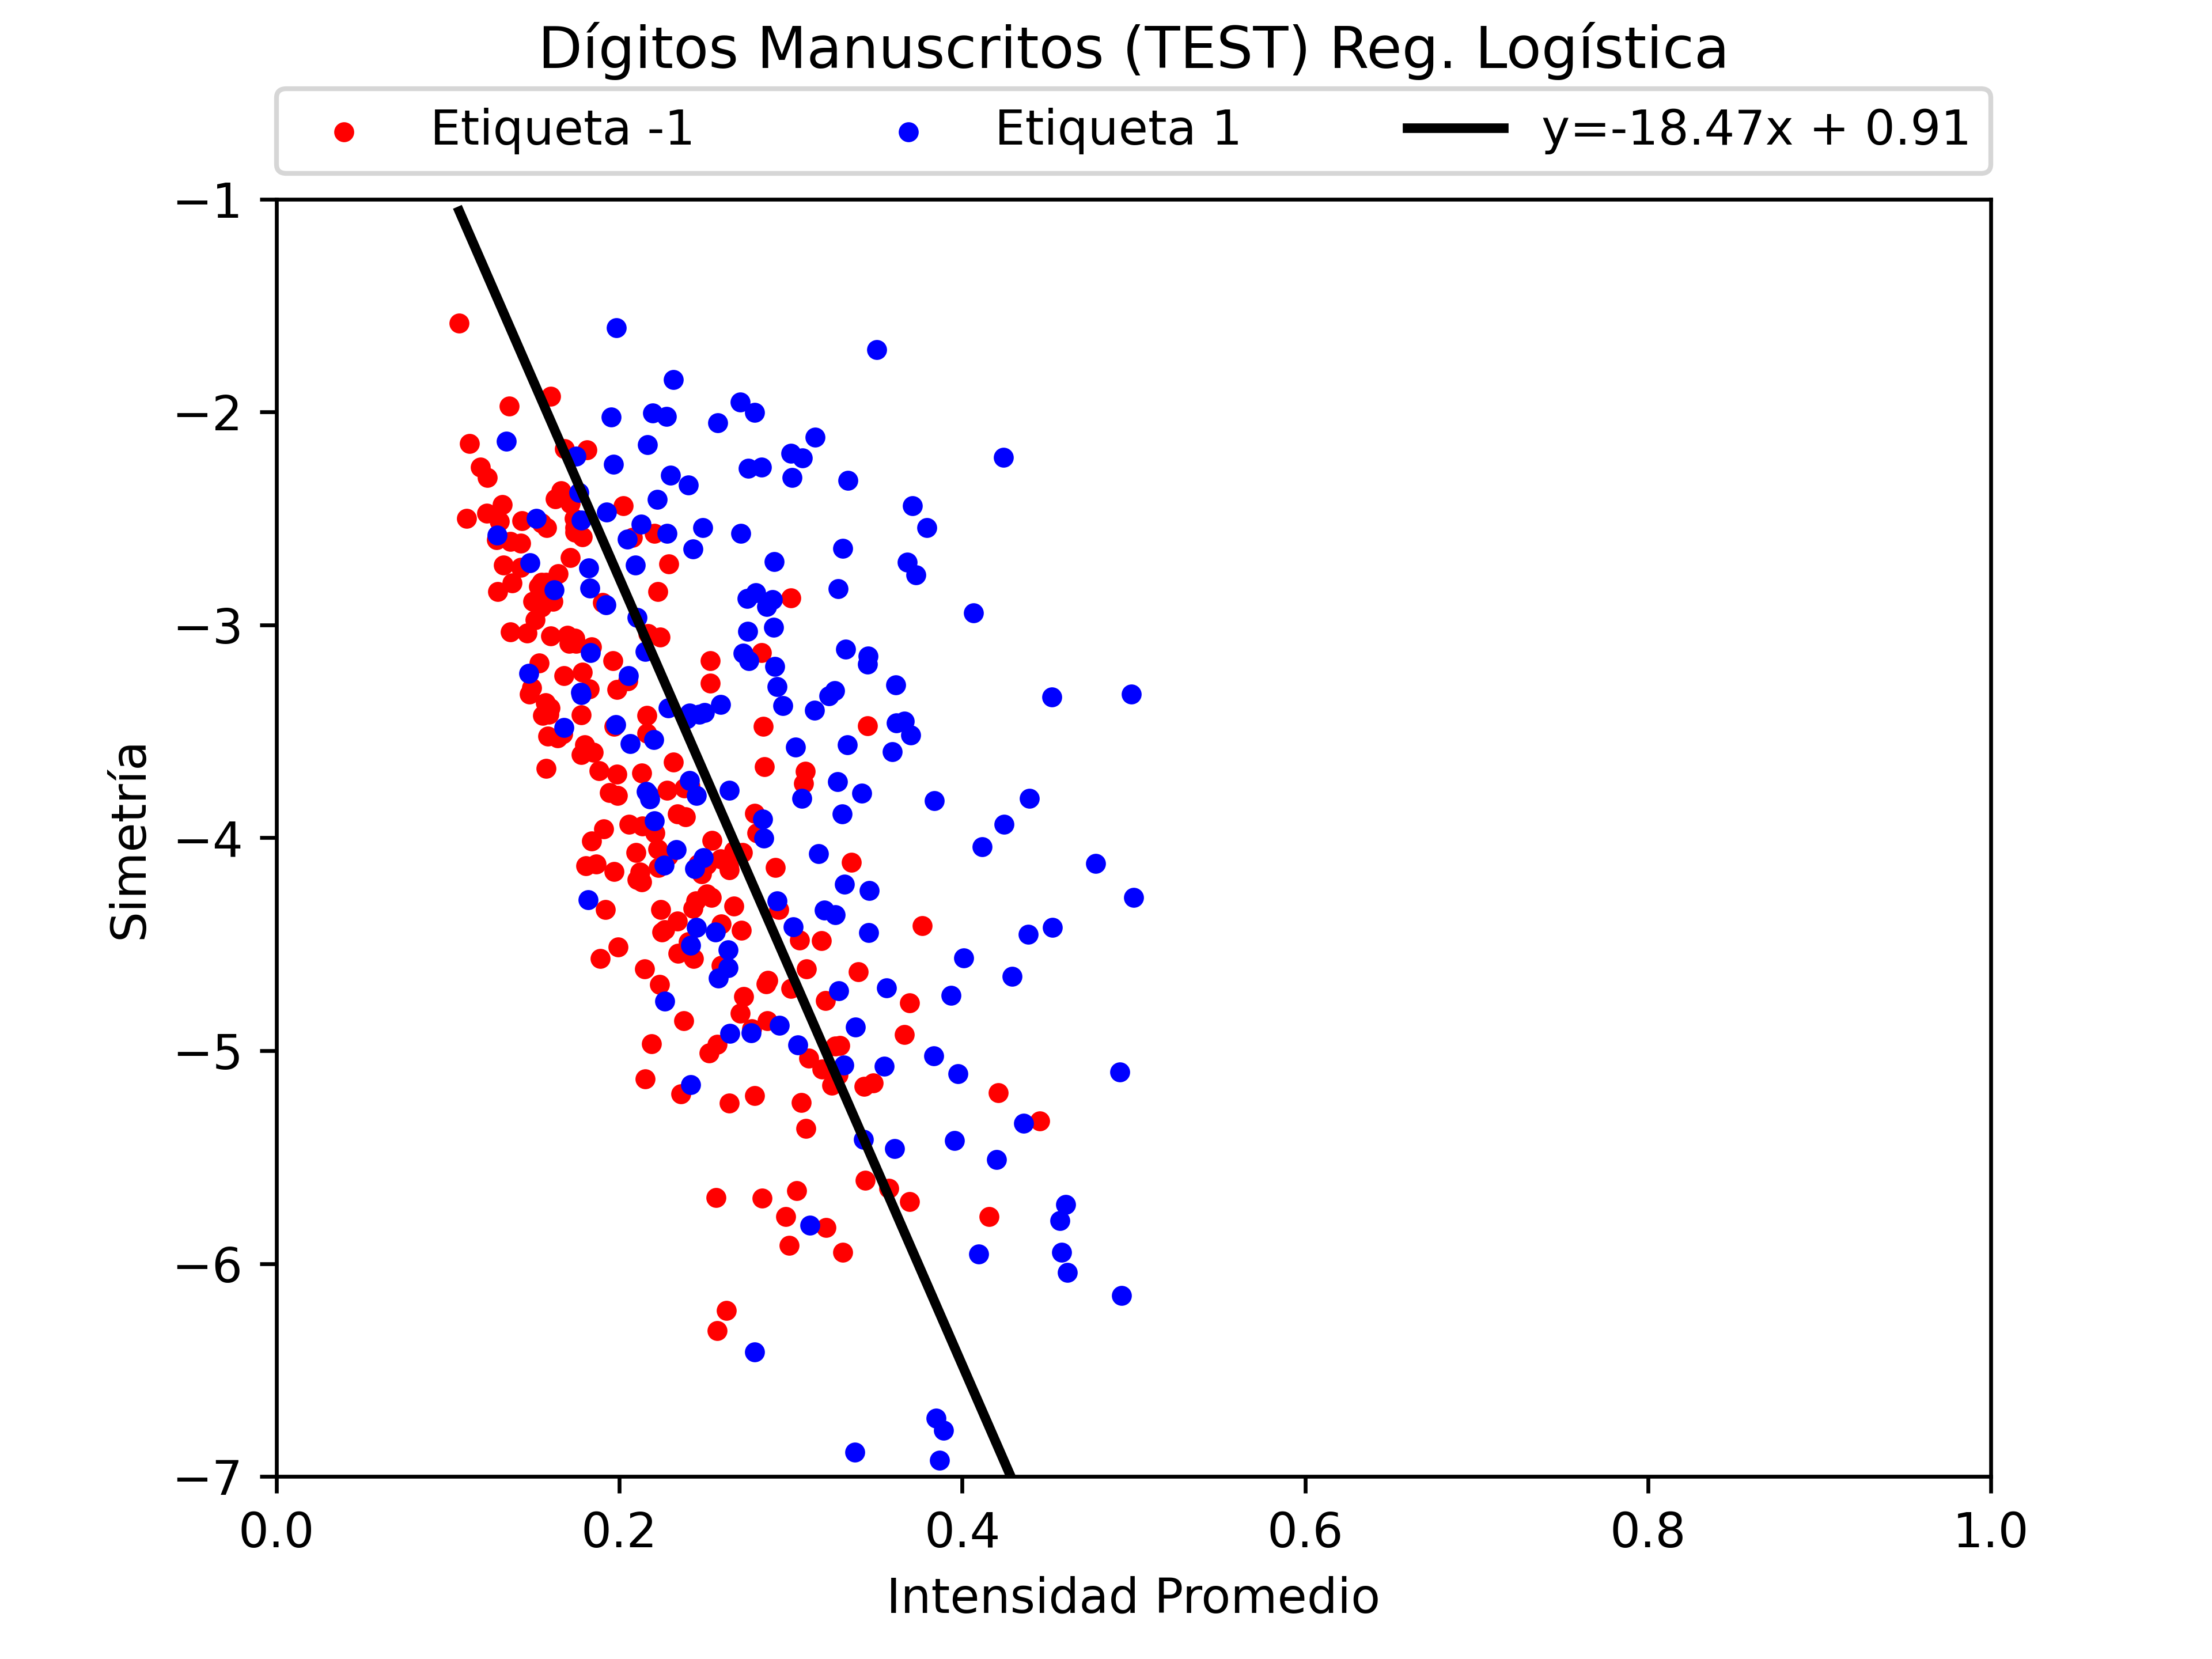
\includegraphics[width=0.9\textwidth]{Figure_20}
      \subcaption{Datos de test}
    \end{minipage}
    \label{fig:dummy64}
\end{figure}



\begin{figure}[H]
    \caption{Algoritmo PLA-POCKET \medskip}
    \begin{minipage}[b]{.5\linewidth}
      \centering
      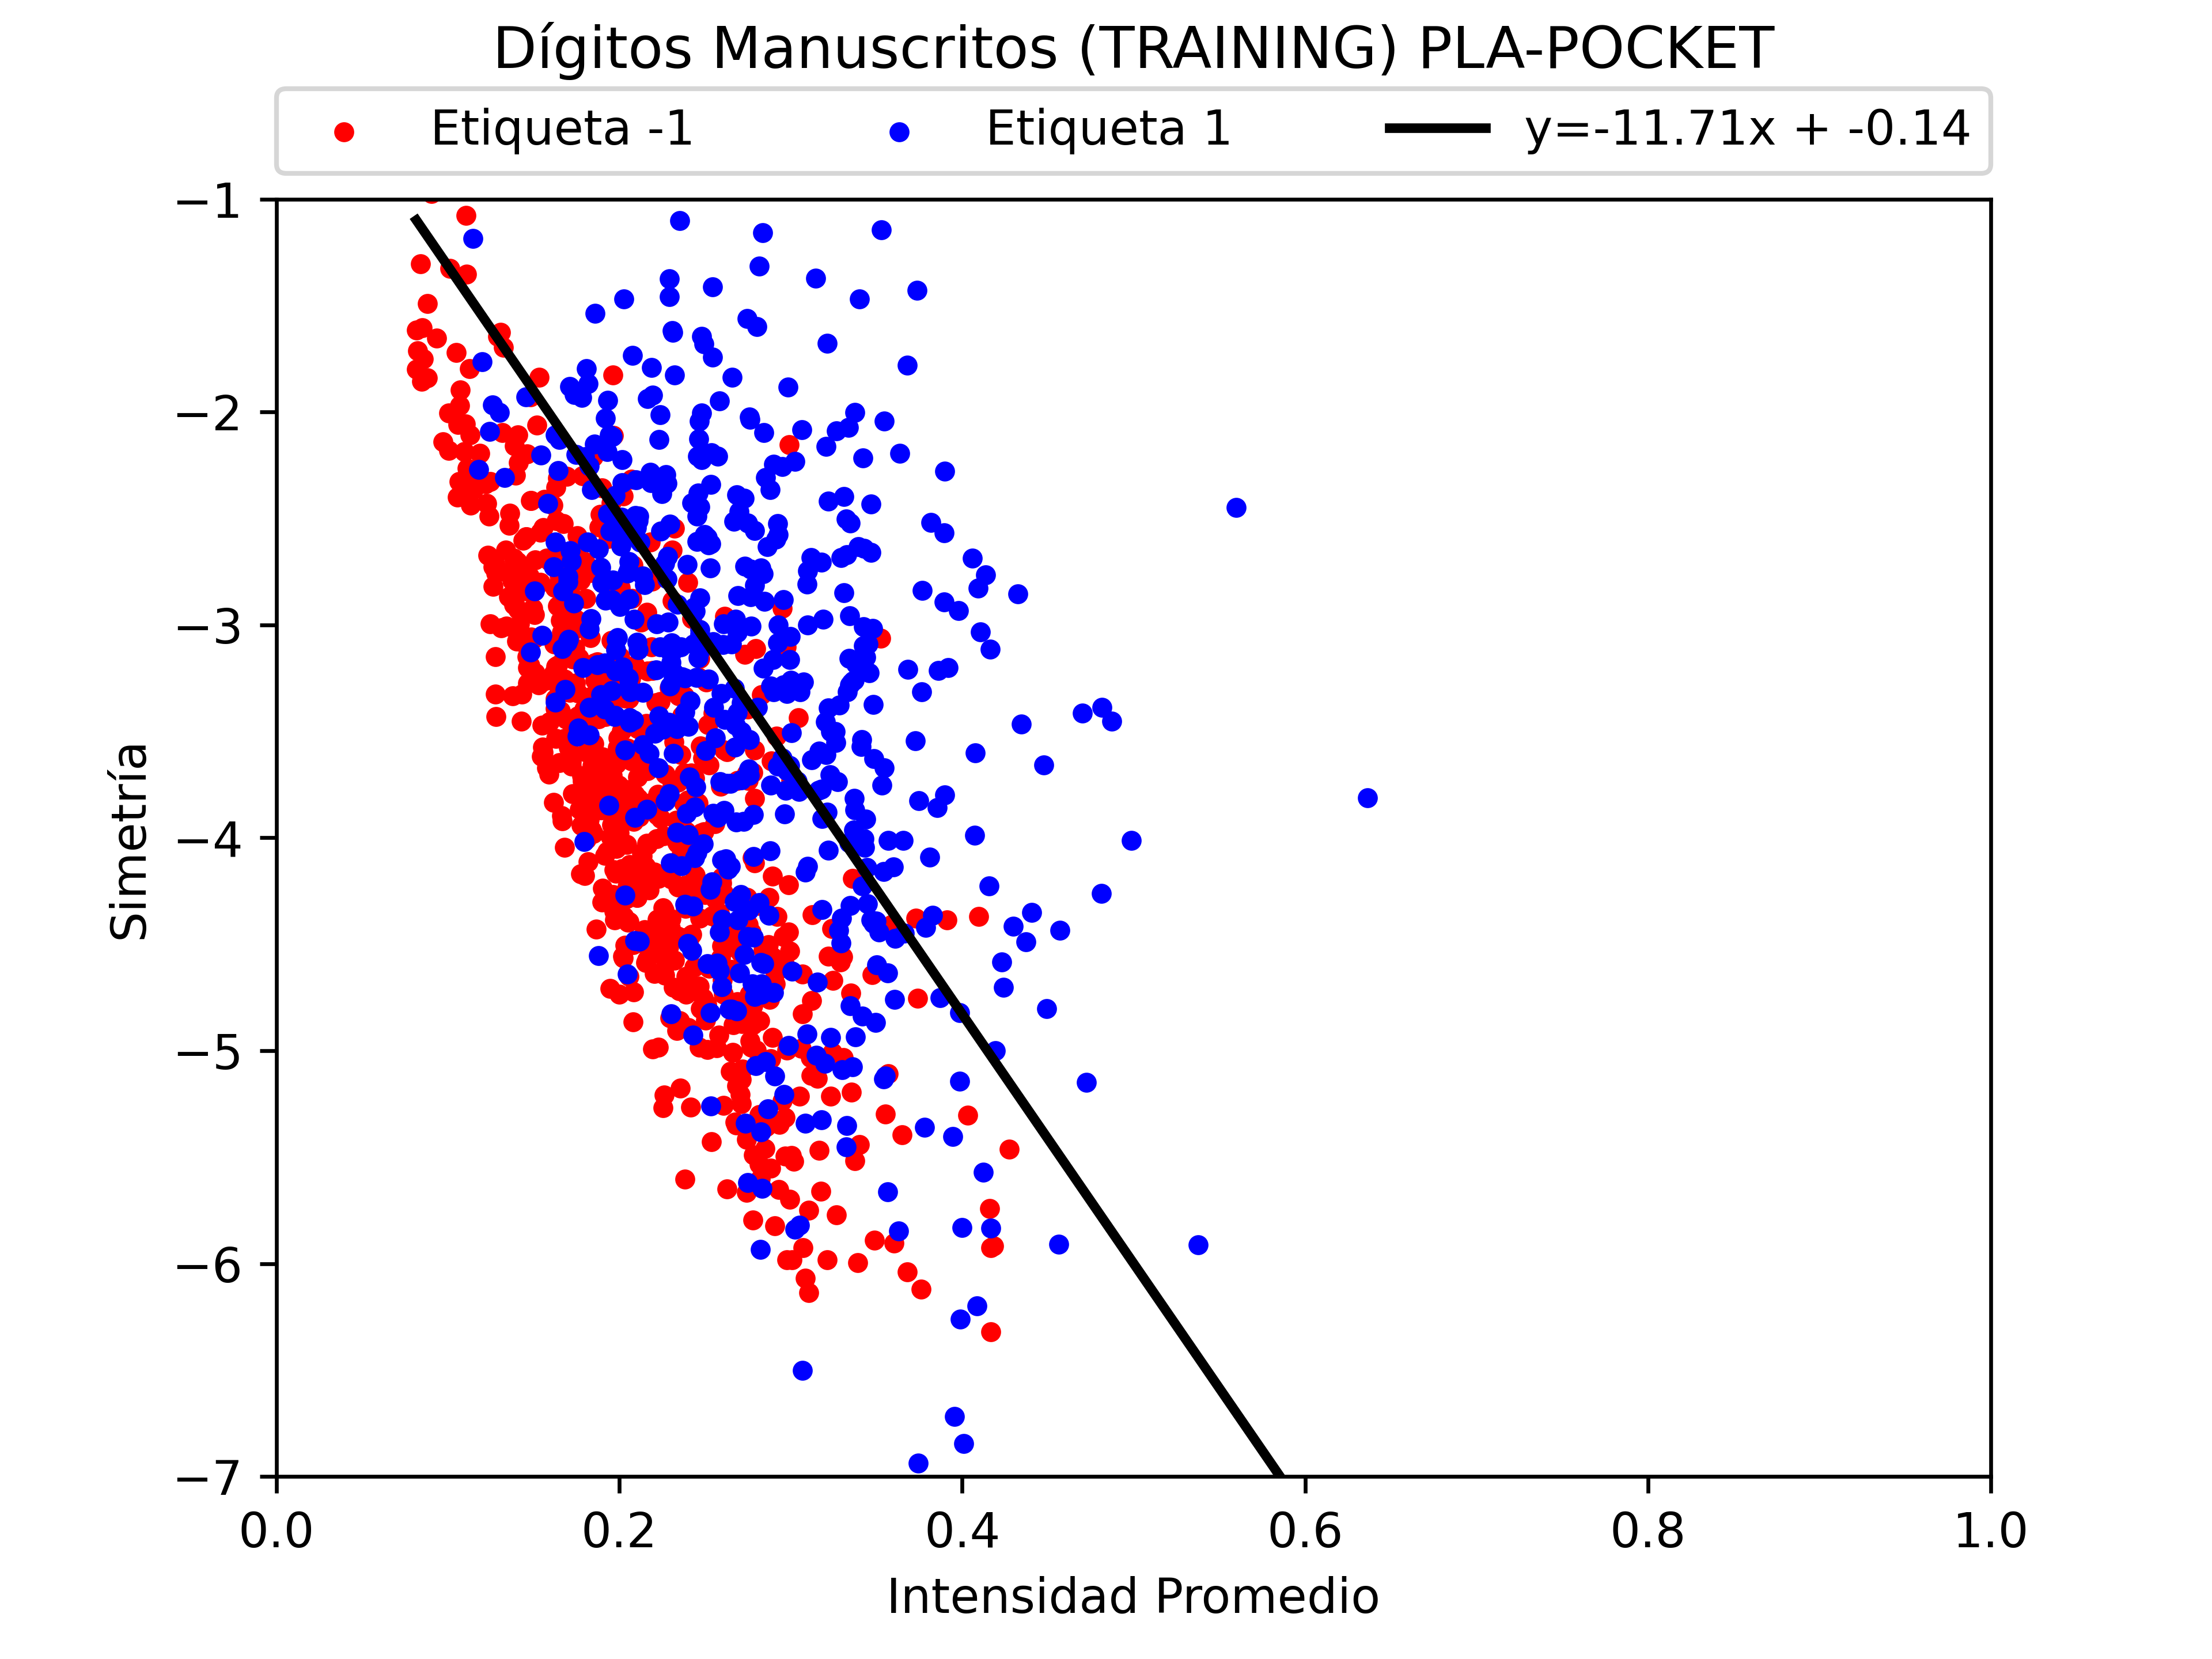
\includegraphics[width=0.9\textwidth]{Figure_21}
      \subcaption{Datos de entrenamiento} \label{subfig-5:dummy65}
    \end{minipage}
    \hfill \hfill
    \begin{minipage}[b]{.5\linewidth}
      \centering
      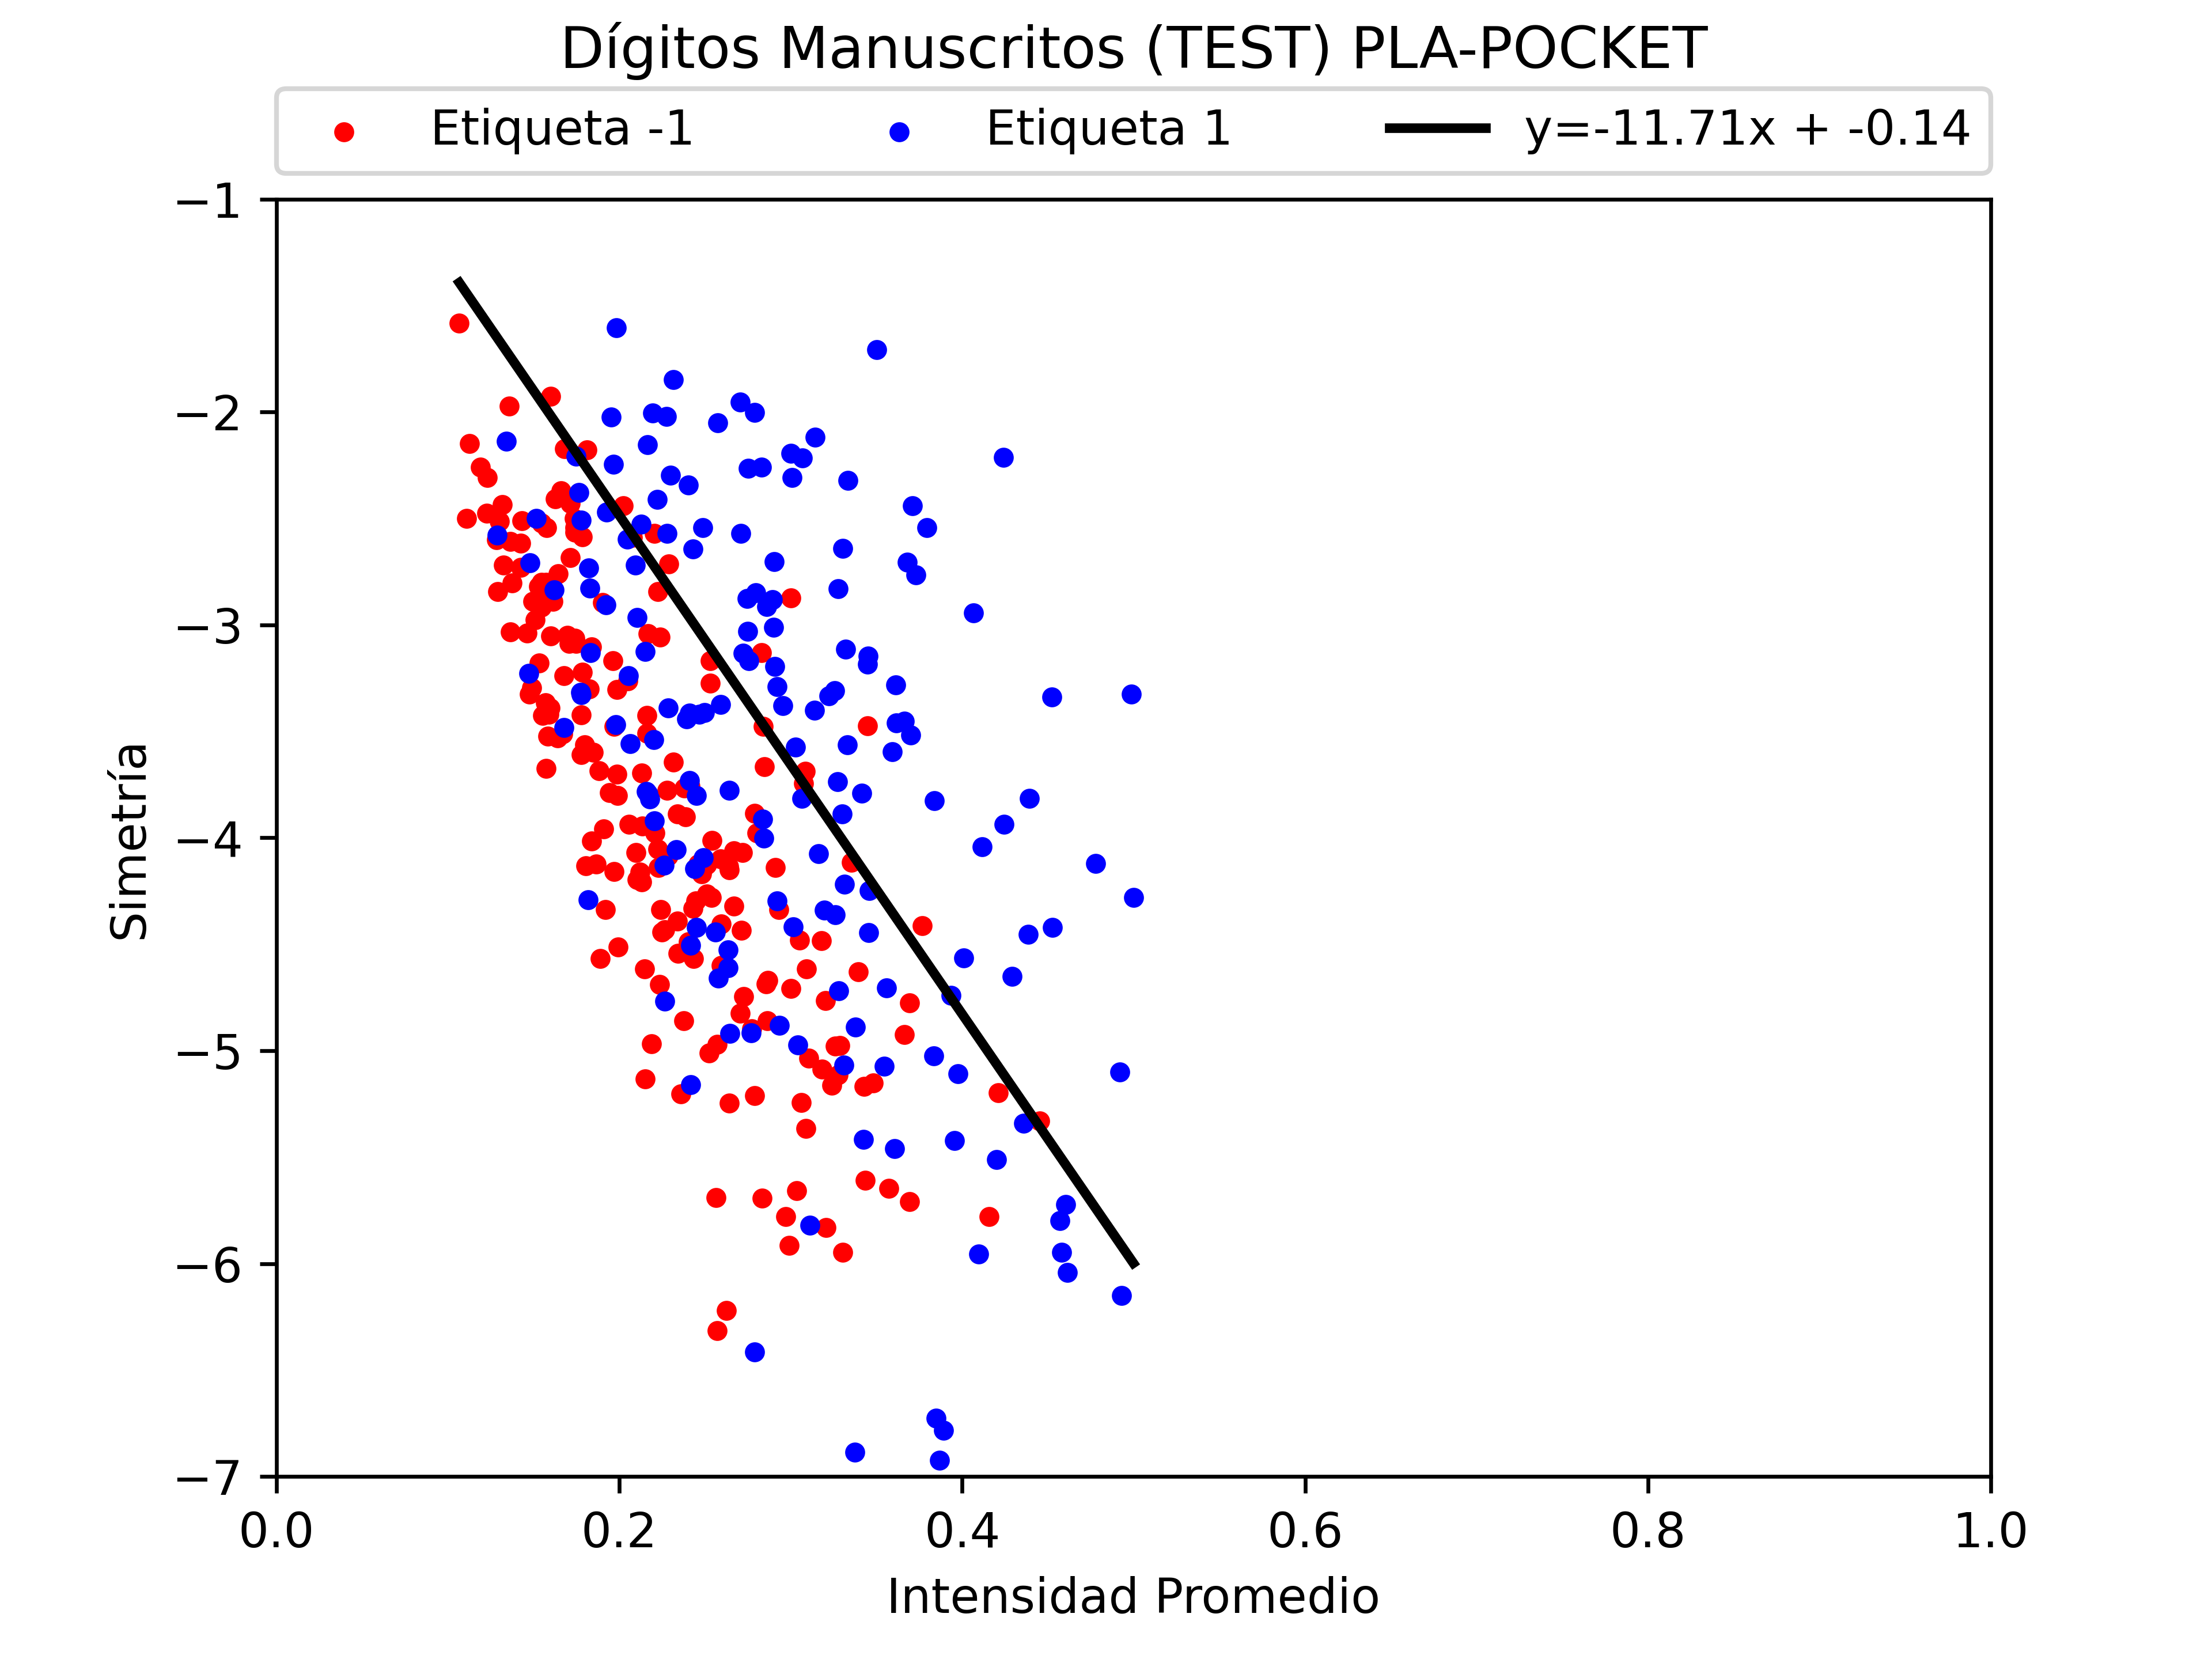
\includegraphics[width=0.9\textwidth]{Figure_22}
      \subcaption{Datos de test}
    \end{minipage}
    \label{fig:dummy65}
\end{figure}

Nos detenemos en \textbf{PLA-POCKET} para comentar que su implementación es
parecida a la de PLA, con la salvedad de que se devuelve el vector de pesos de
salida que mejor $E_{in}$ proporcione en las iteraciones. Es decir, se reemplaza
sucesivamente $w$ si se calcula otro con menor error \textit{in-sample} asociado.

\subsection{Calcular $E_{in}$ y $E_{test}$}

\begin{table}[H]
    \centering
    \begin{tabular}{llllll} \toprule
        Algoritmo & $E_{in}$ & $E_{test}$ & $E_{in}^{clas}$ (\%) & $E_{test}^{clas}$ (\%) & Iteraciones \\ \midrule
        Regresión Lineal& $0.643$ & $0.709$ & $22.8 \%$ & $25.1 \%$ & ----- \\ 
        PLA & $0.309$ & $0.301$ & $30.9 \%$ & $30.1 \%$ & $1000$ \\ 
        Regresión Logística & $0.464$ & $0.527$ & $22.2 \%$ & $26.0 \%$ & $552$ \\ 
        PLA-POCKET & $0.264$ & $0.281$ & $26.4 \%$ & $28.1 \%$ & $36$ \\ \bottomrule
    \end{tabular}
    \caption{Comparación de los modelos lineales estudiados}
\end{table}

\subsection{Repetir inicialización con los pesos obtenidos mediante regresión lineal}

\textbf{Si se emplean los pesos obtenidos con regresión lineal para inicializar
los otros tres métodos (RL, PLA, PLA-pocket), ¿se observa alguna mejora en
los resultados a algún nivel? Justifique su respuesta}

Denominamos $w_{lin}$ a los pesos obtenidos tras aplicar regresión lineal al conjunto
de datos de entrenamiento.

\begin{figure}[H]
    \caption{PLA inicializado con $w_{lin}$ \medskip}
    \begin{minipage}[b]{.5\linewidth}
      \centering
      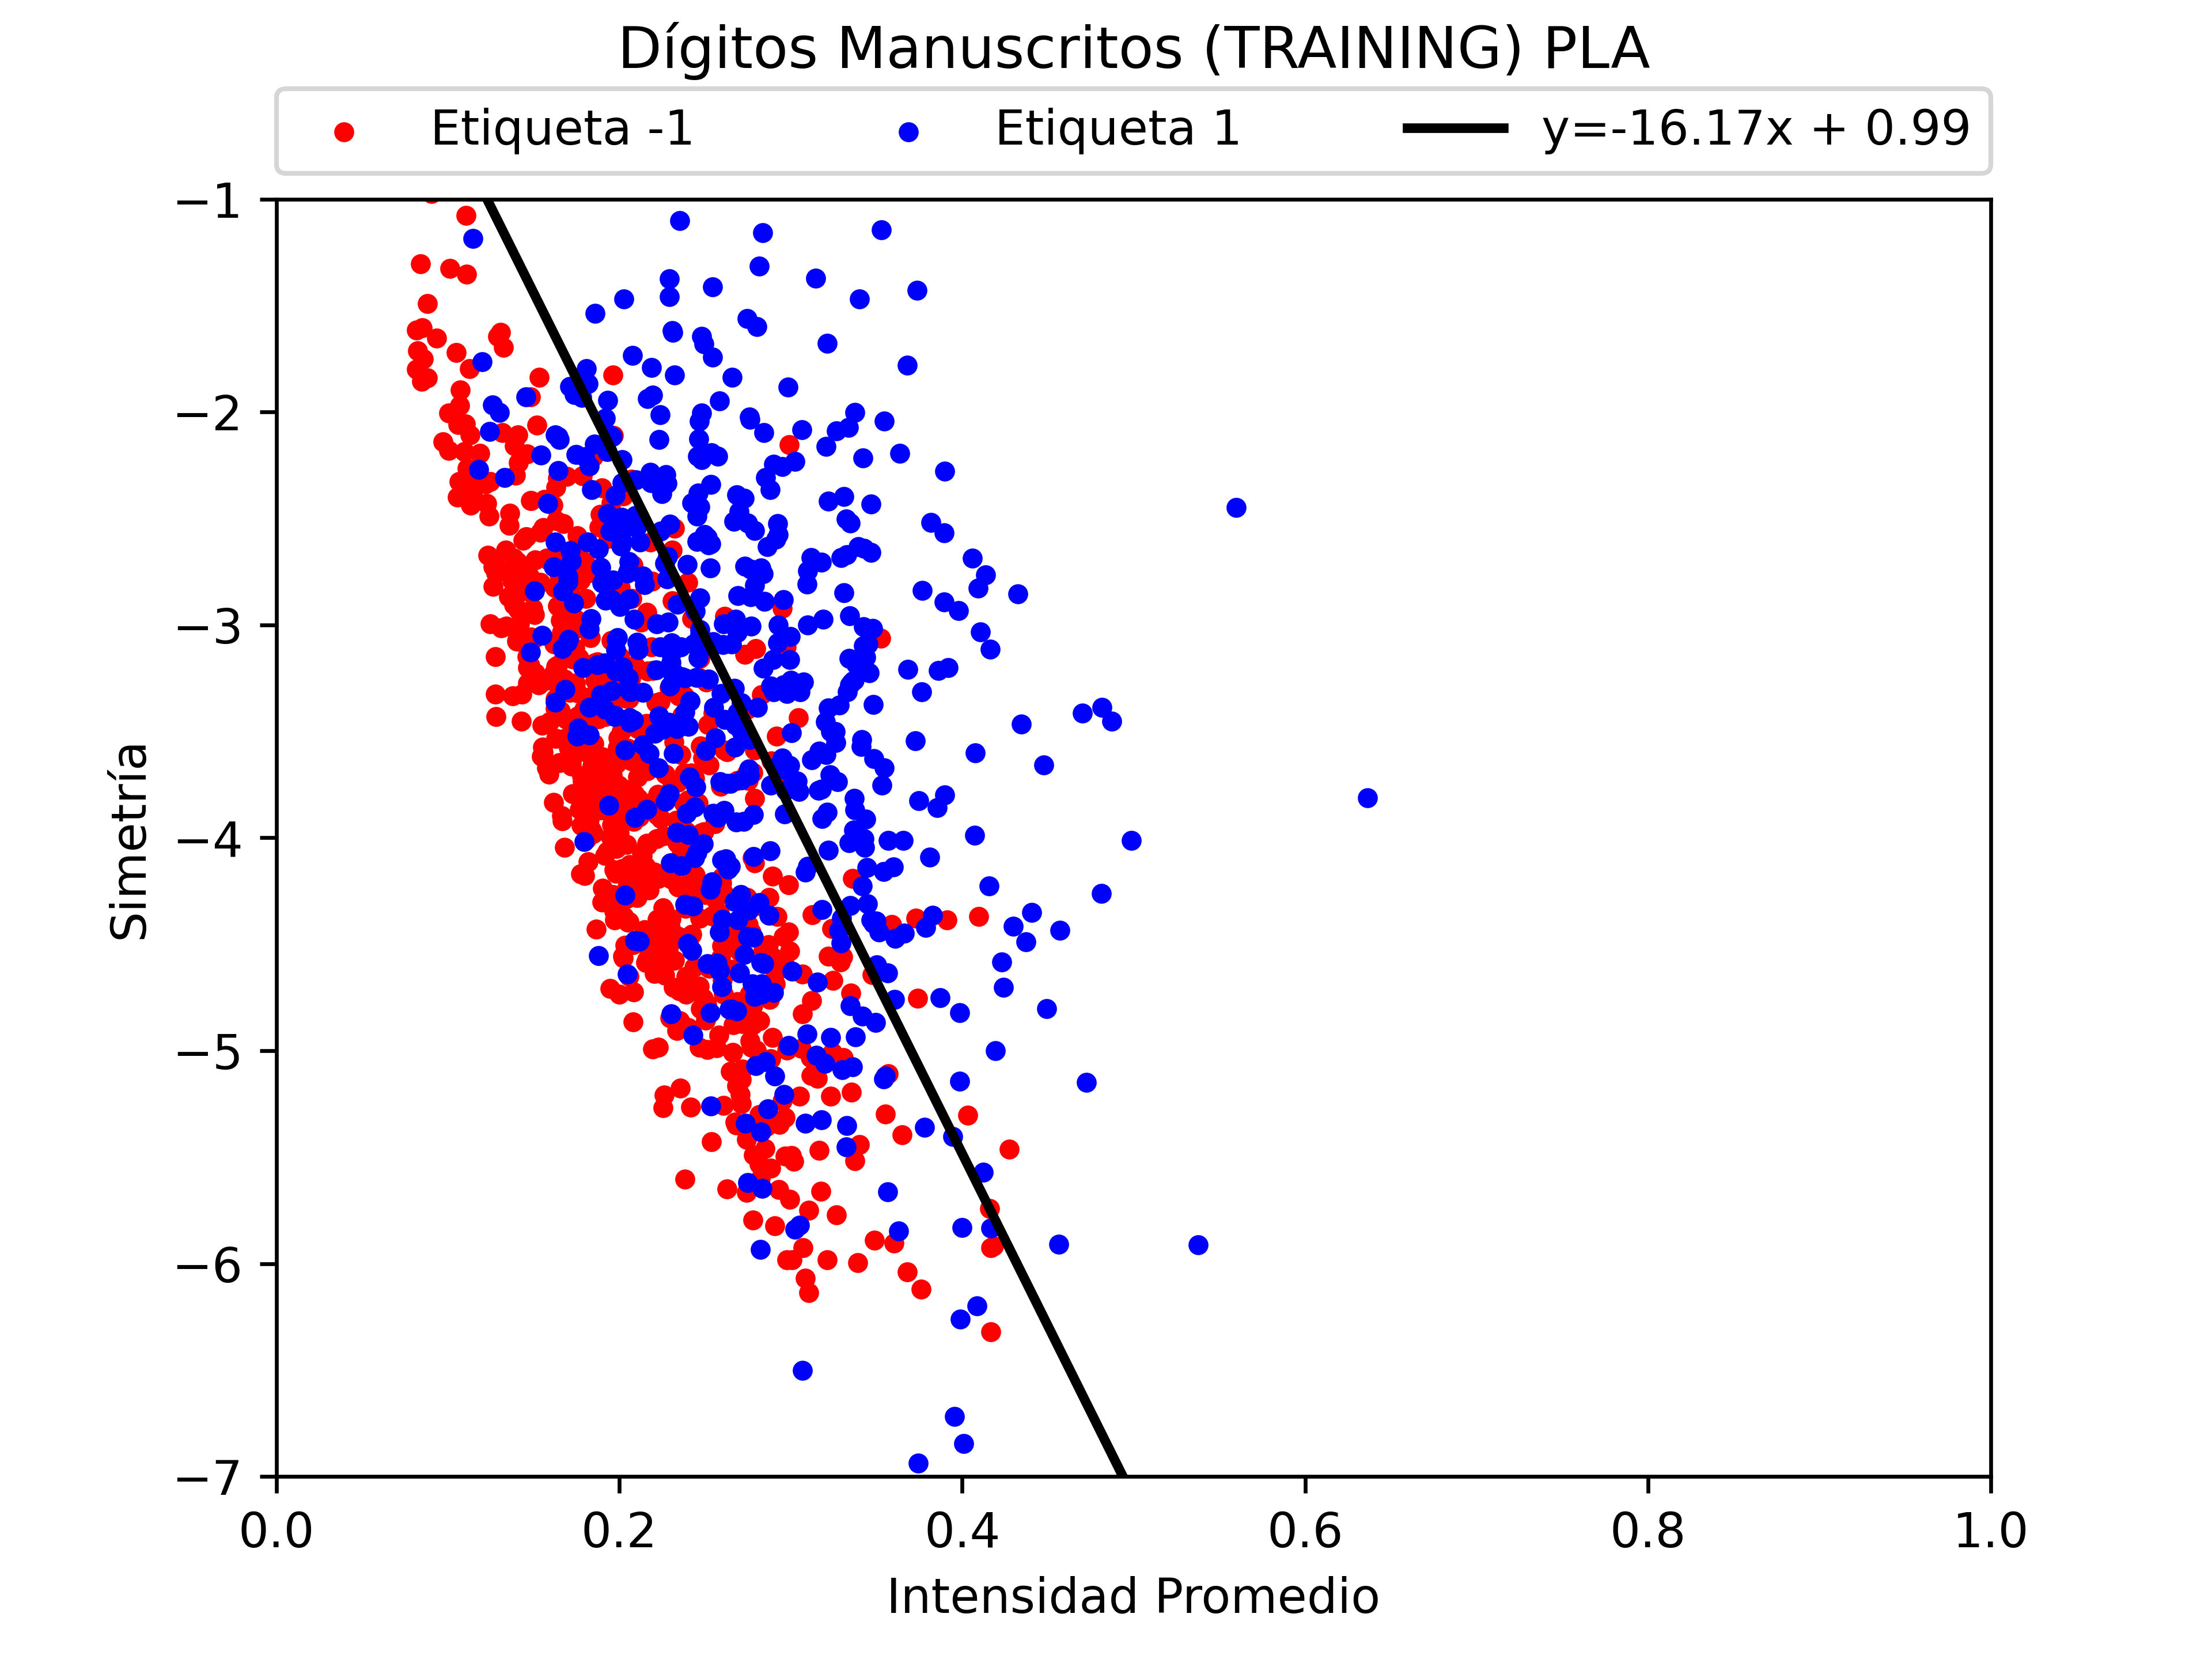
\includegraphics[width=0.9\textwidth]{Figure_23}
      \subcaption{Datos de entrenamiento} \label{subfig-5:dummy66}
    \end{minipage}
    \hfill \hfill
    \begin{minipage}[b]{.5\linewidth}
      \centering
      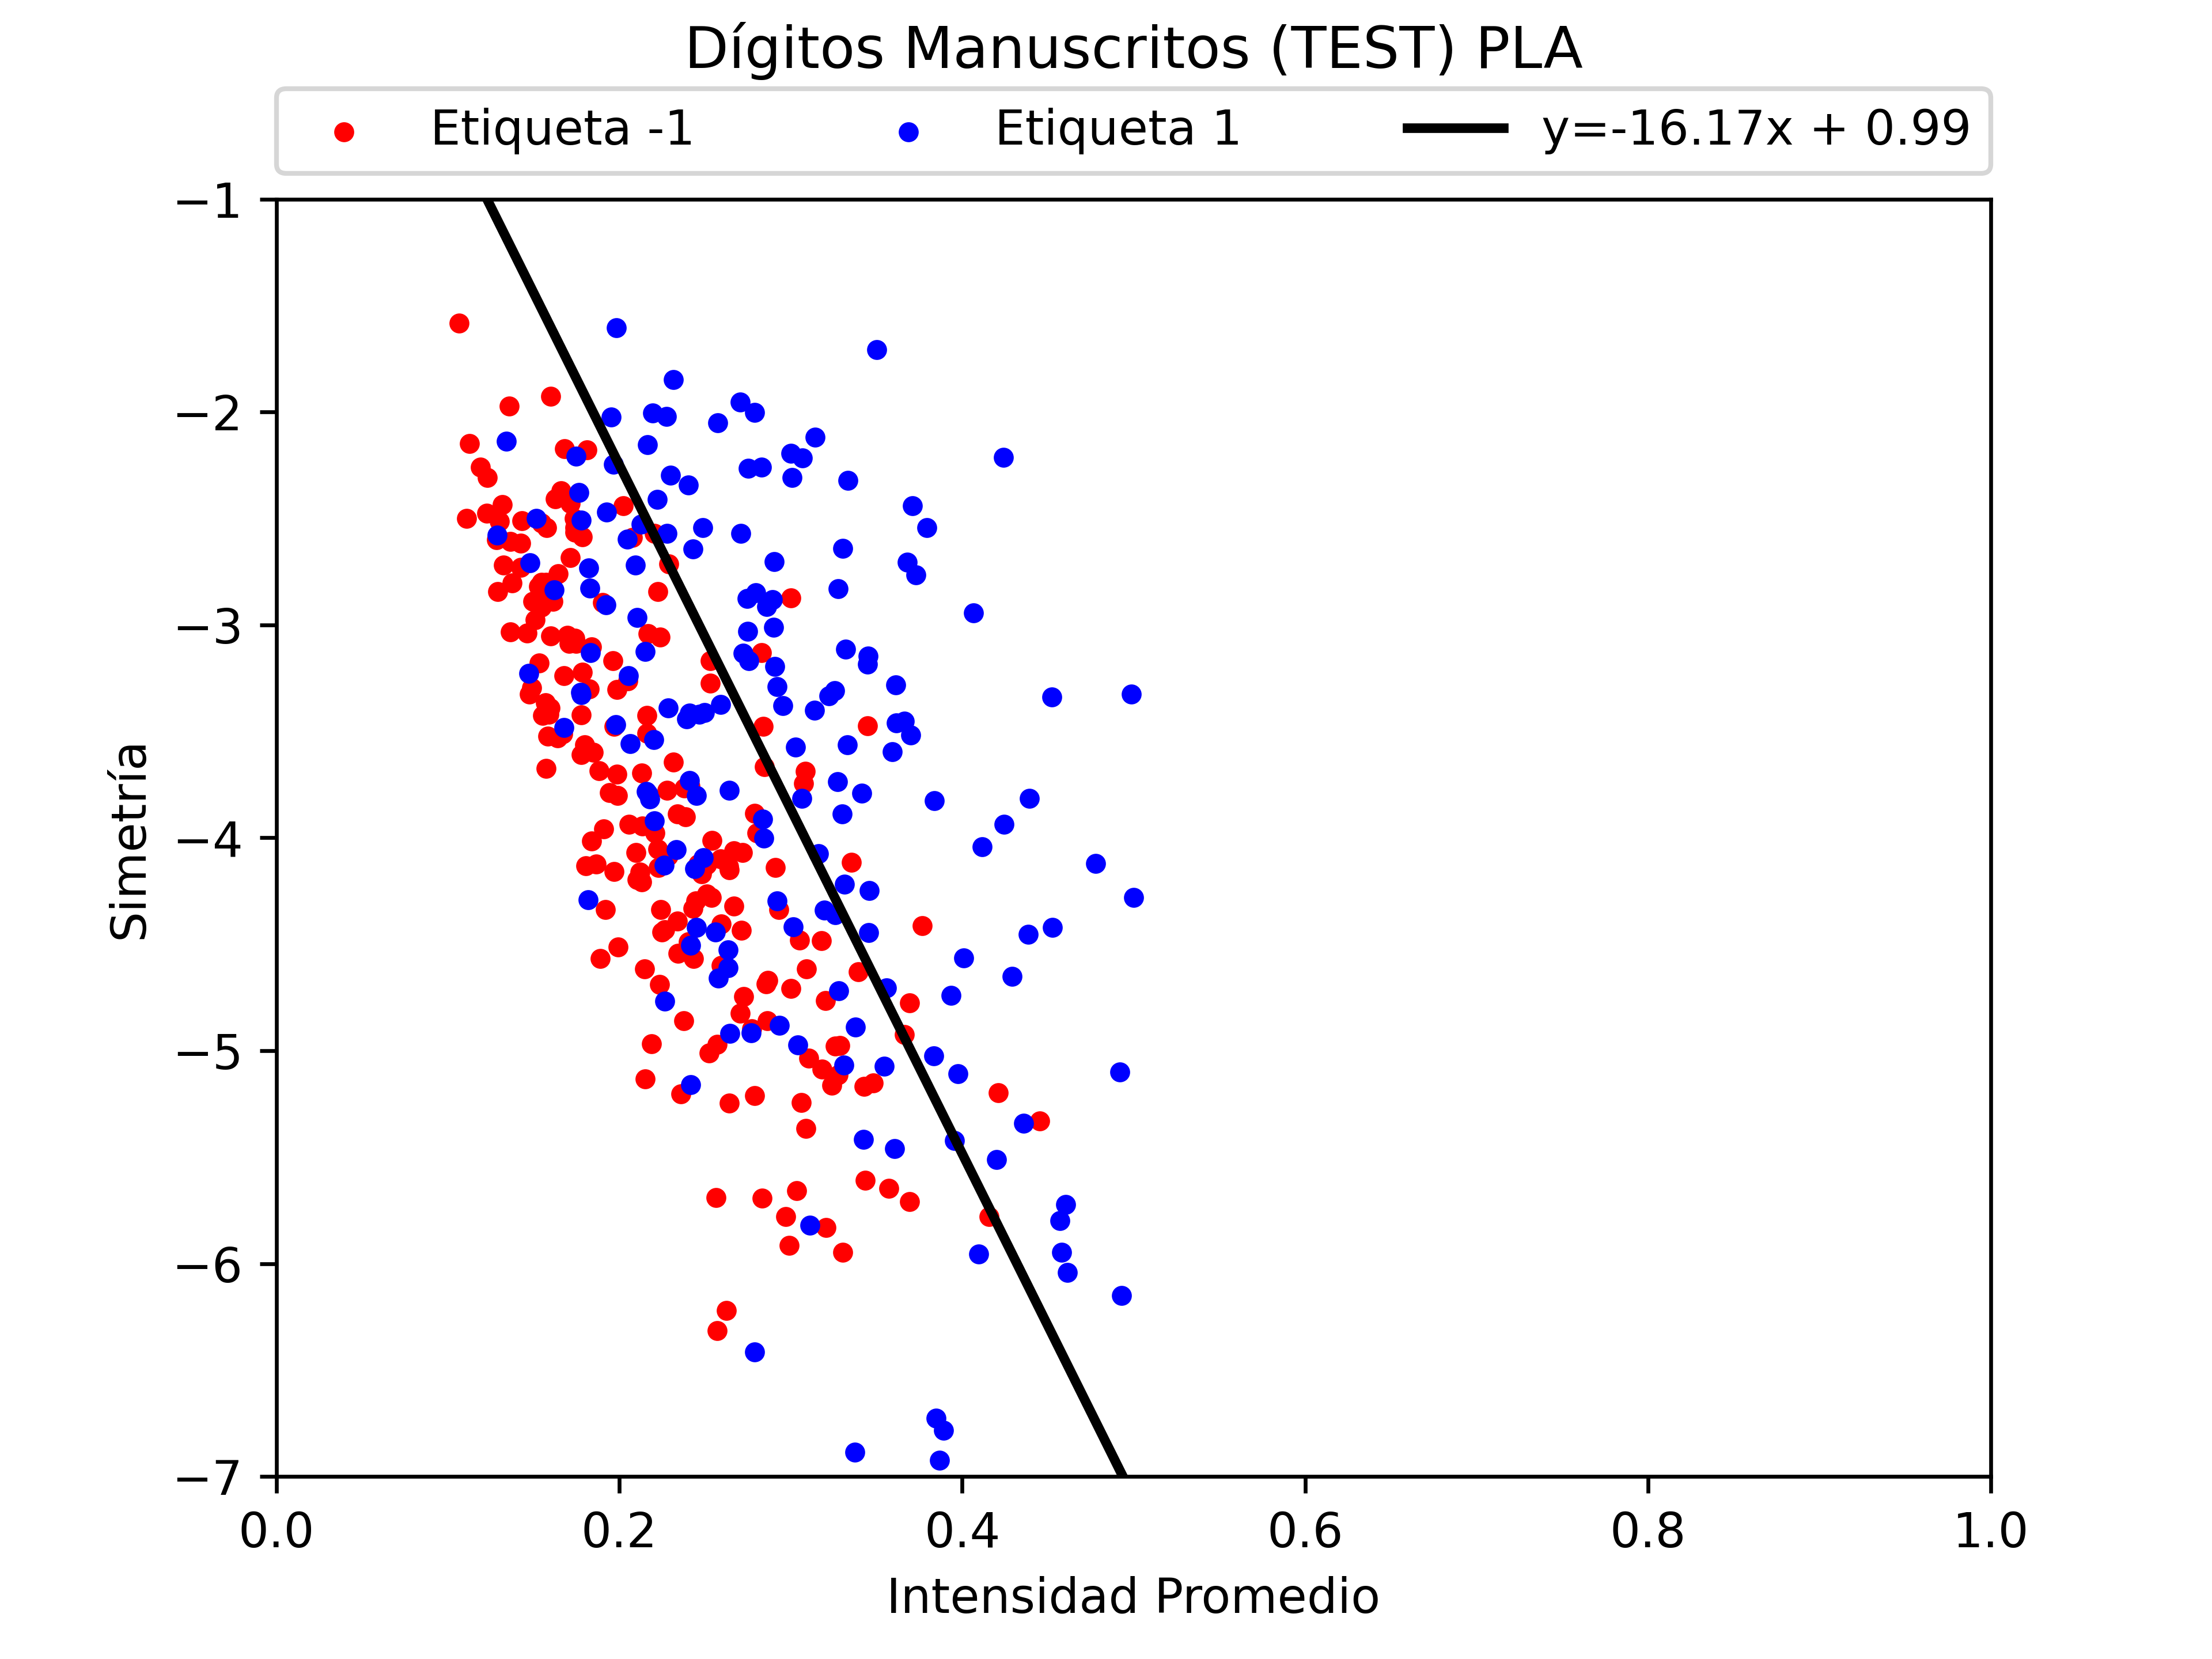
\includegraphics[width=0.9\textwidth]{Figure_24}
      \subcaption{Datos de test}
    \end{minipage}
    \label{fig:dummy66}
\end{figure}

\begin{figure}[H]
    \caption{RL inicializado con $w_{lin}$ \medskip}
    \begin{minipage}[b]{.5\linewidth}
      \centering
      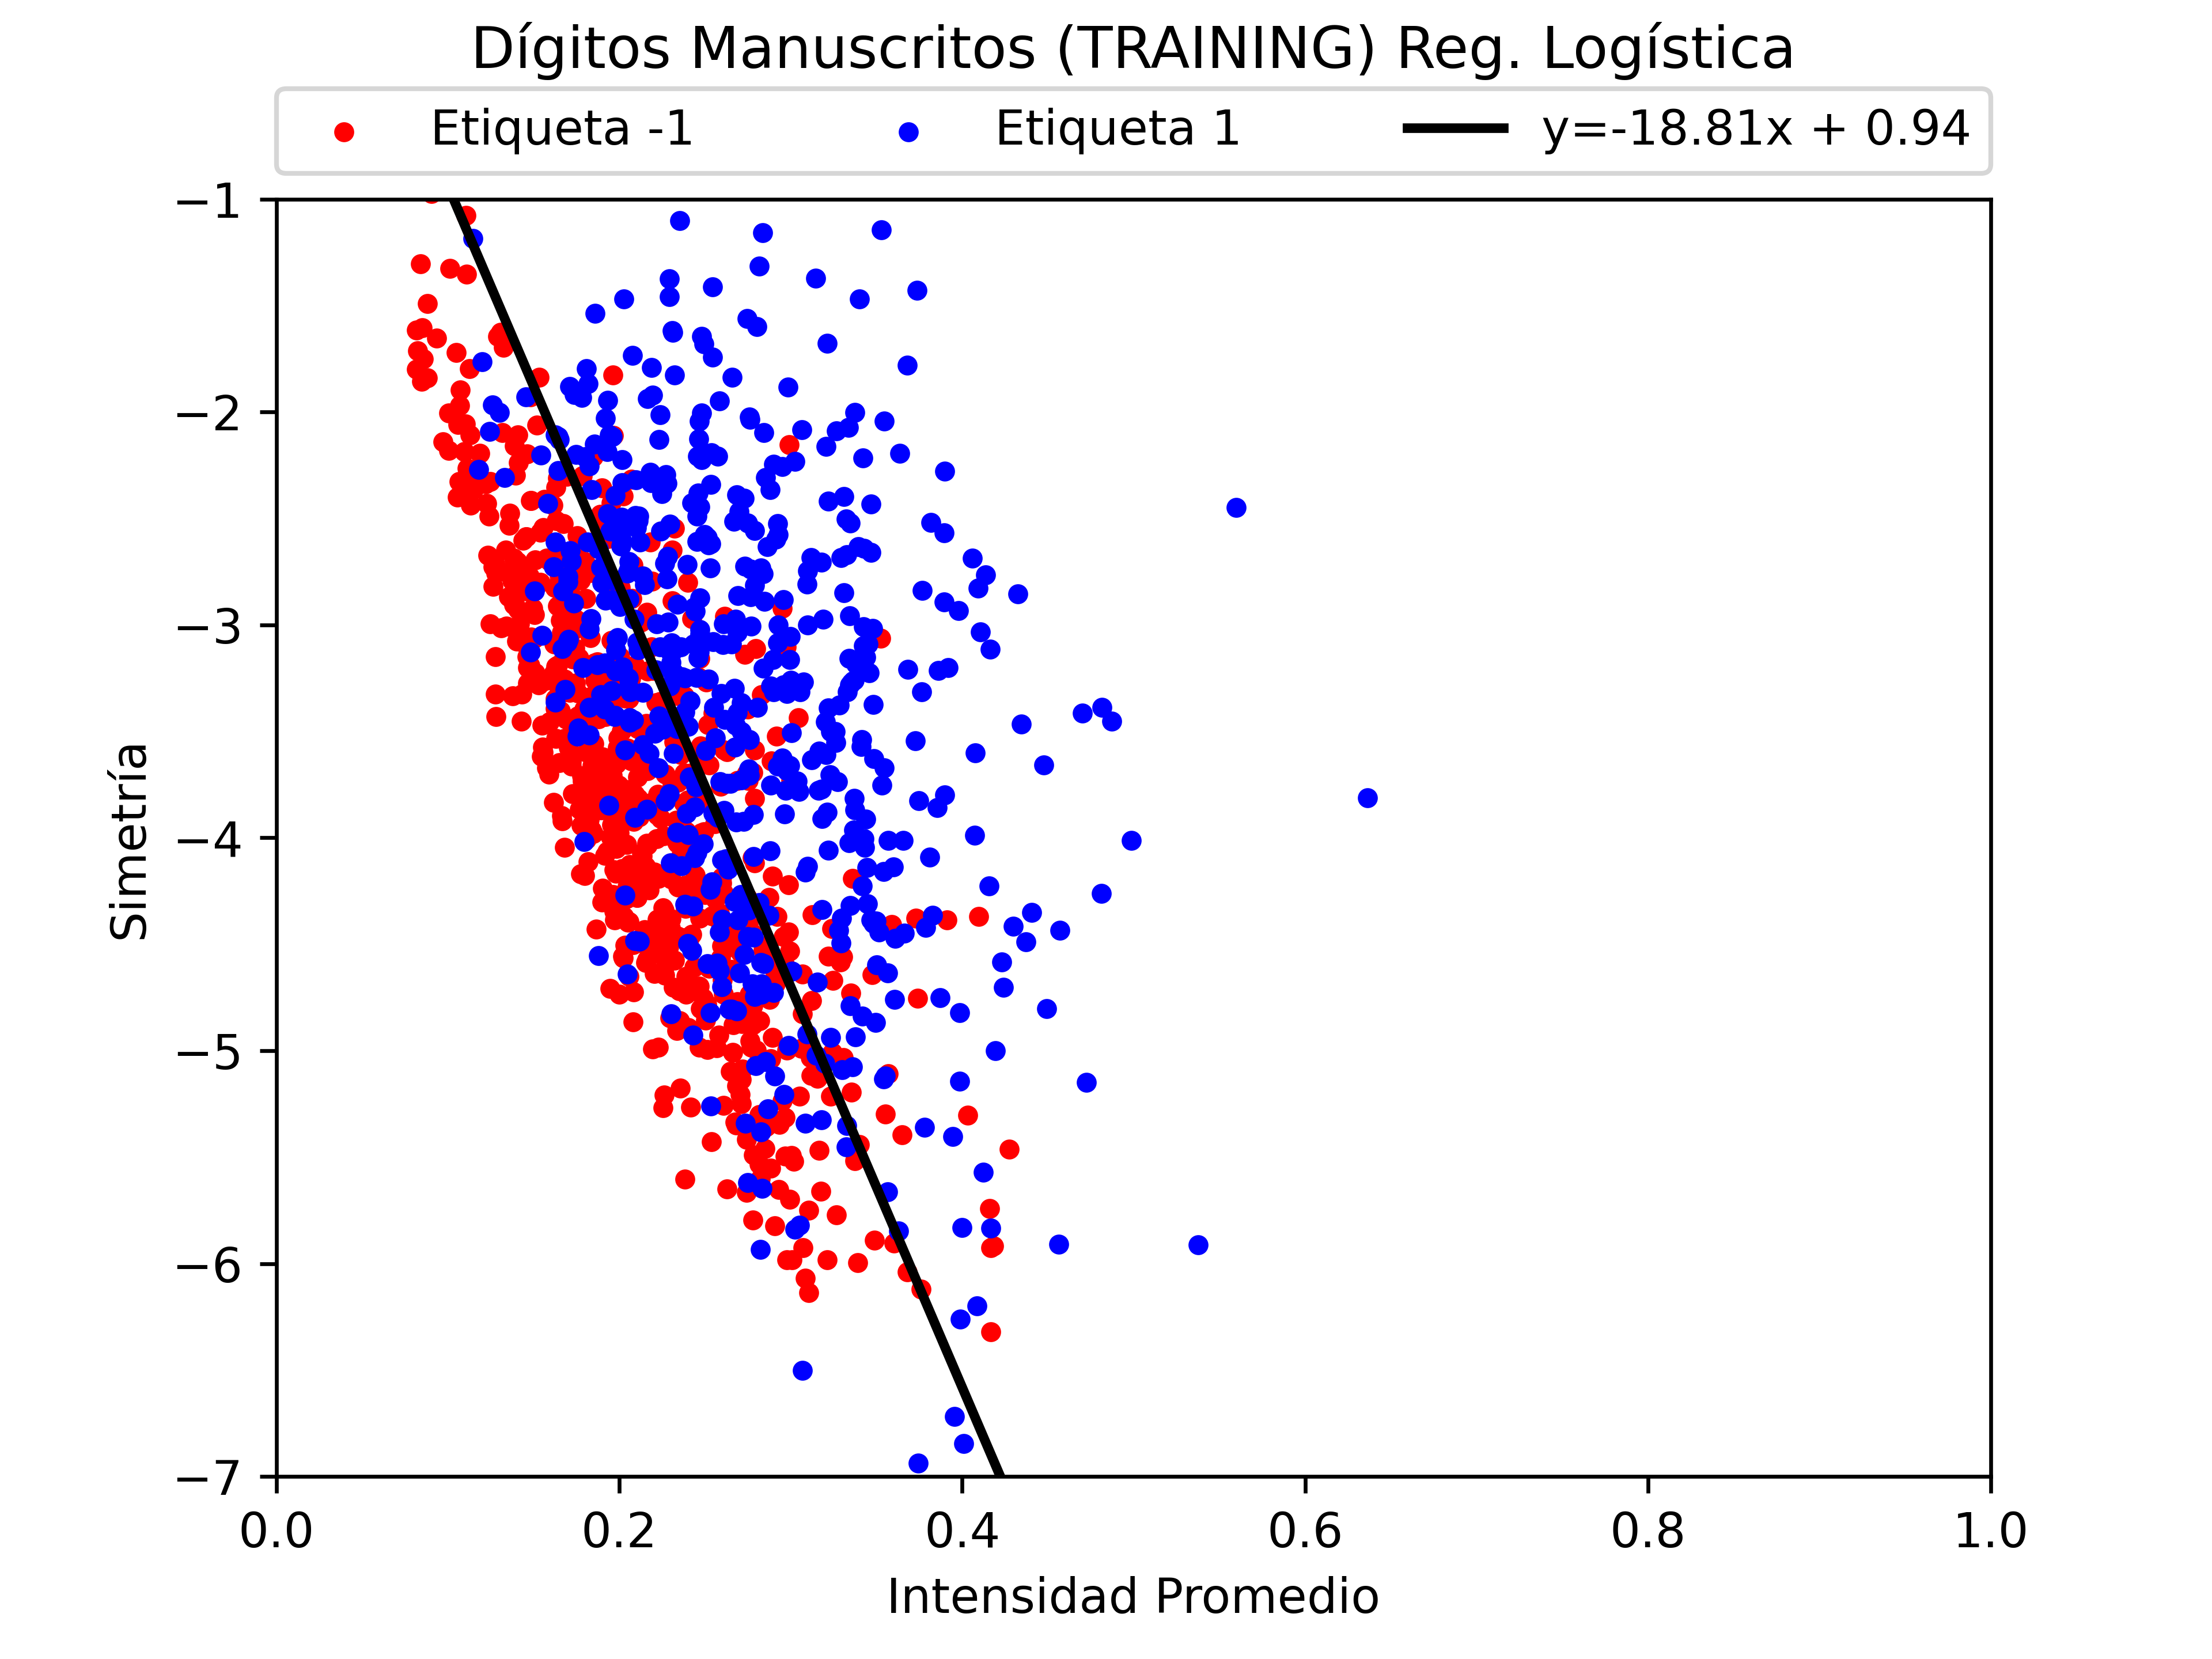
\includegraphics[width=0.9\textwidth]{Figure_25}
      \subcaption{Datos de entrenamiento} \label{subfig-5:dummy67}
    \end{minipage}
    \hfill \hfill
    \begin{minipage}[b]{.5\linewidth}
      \centering
      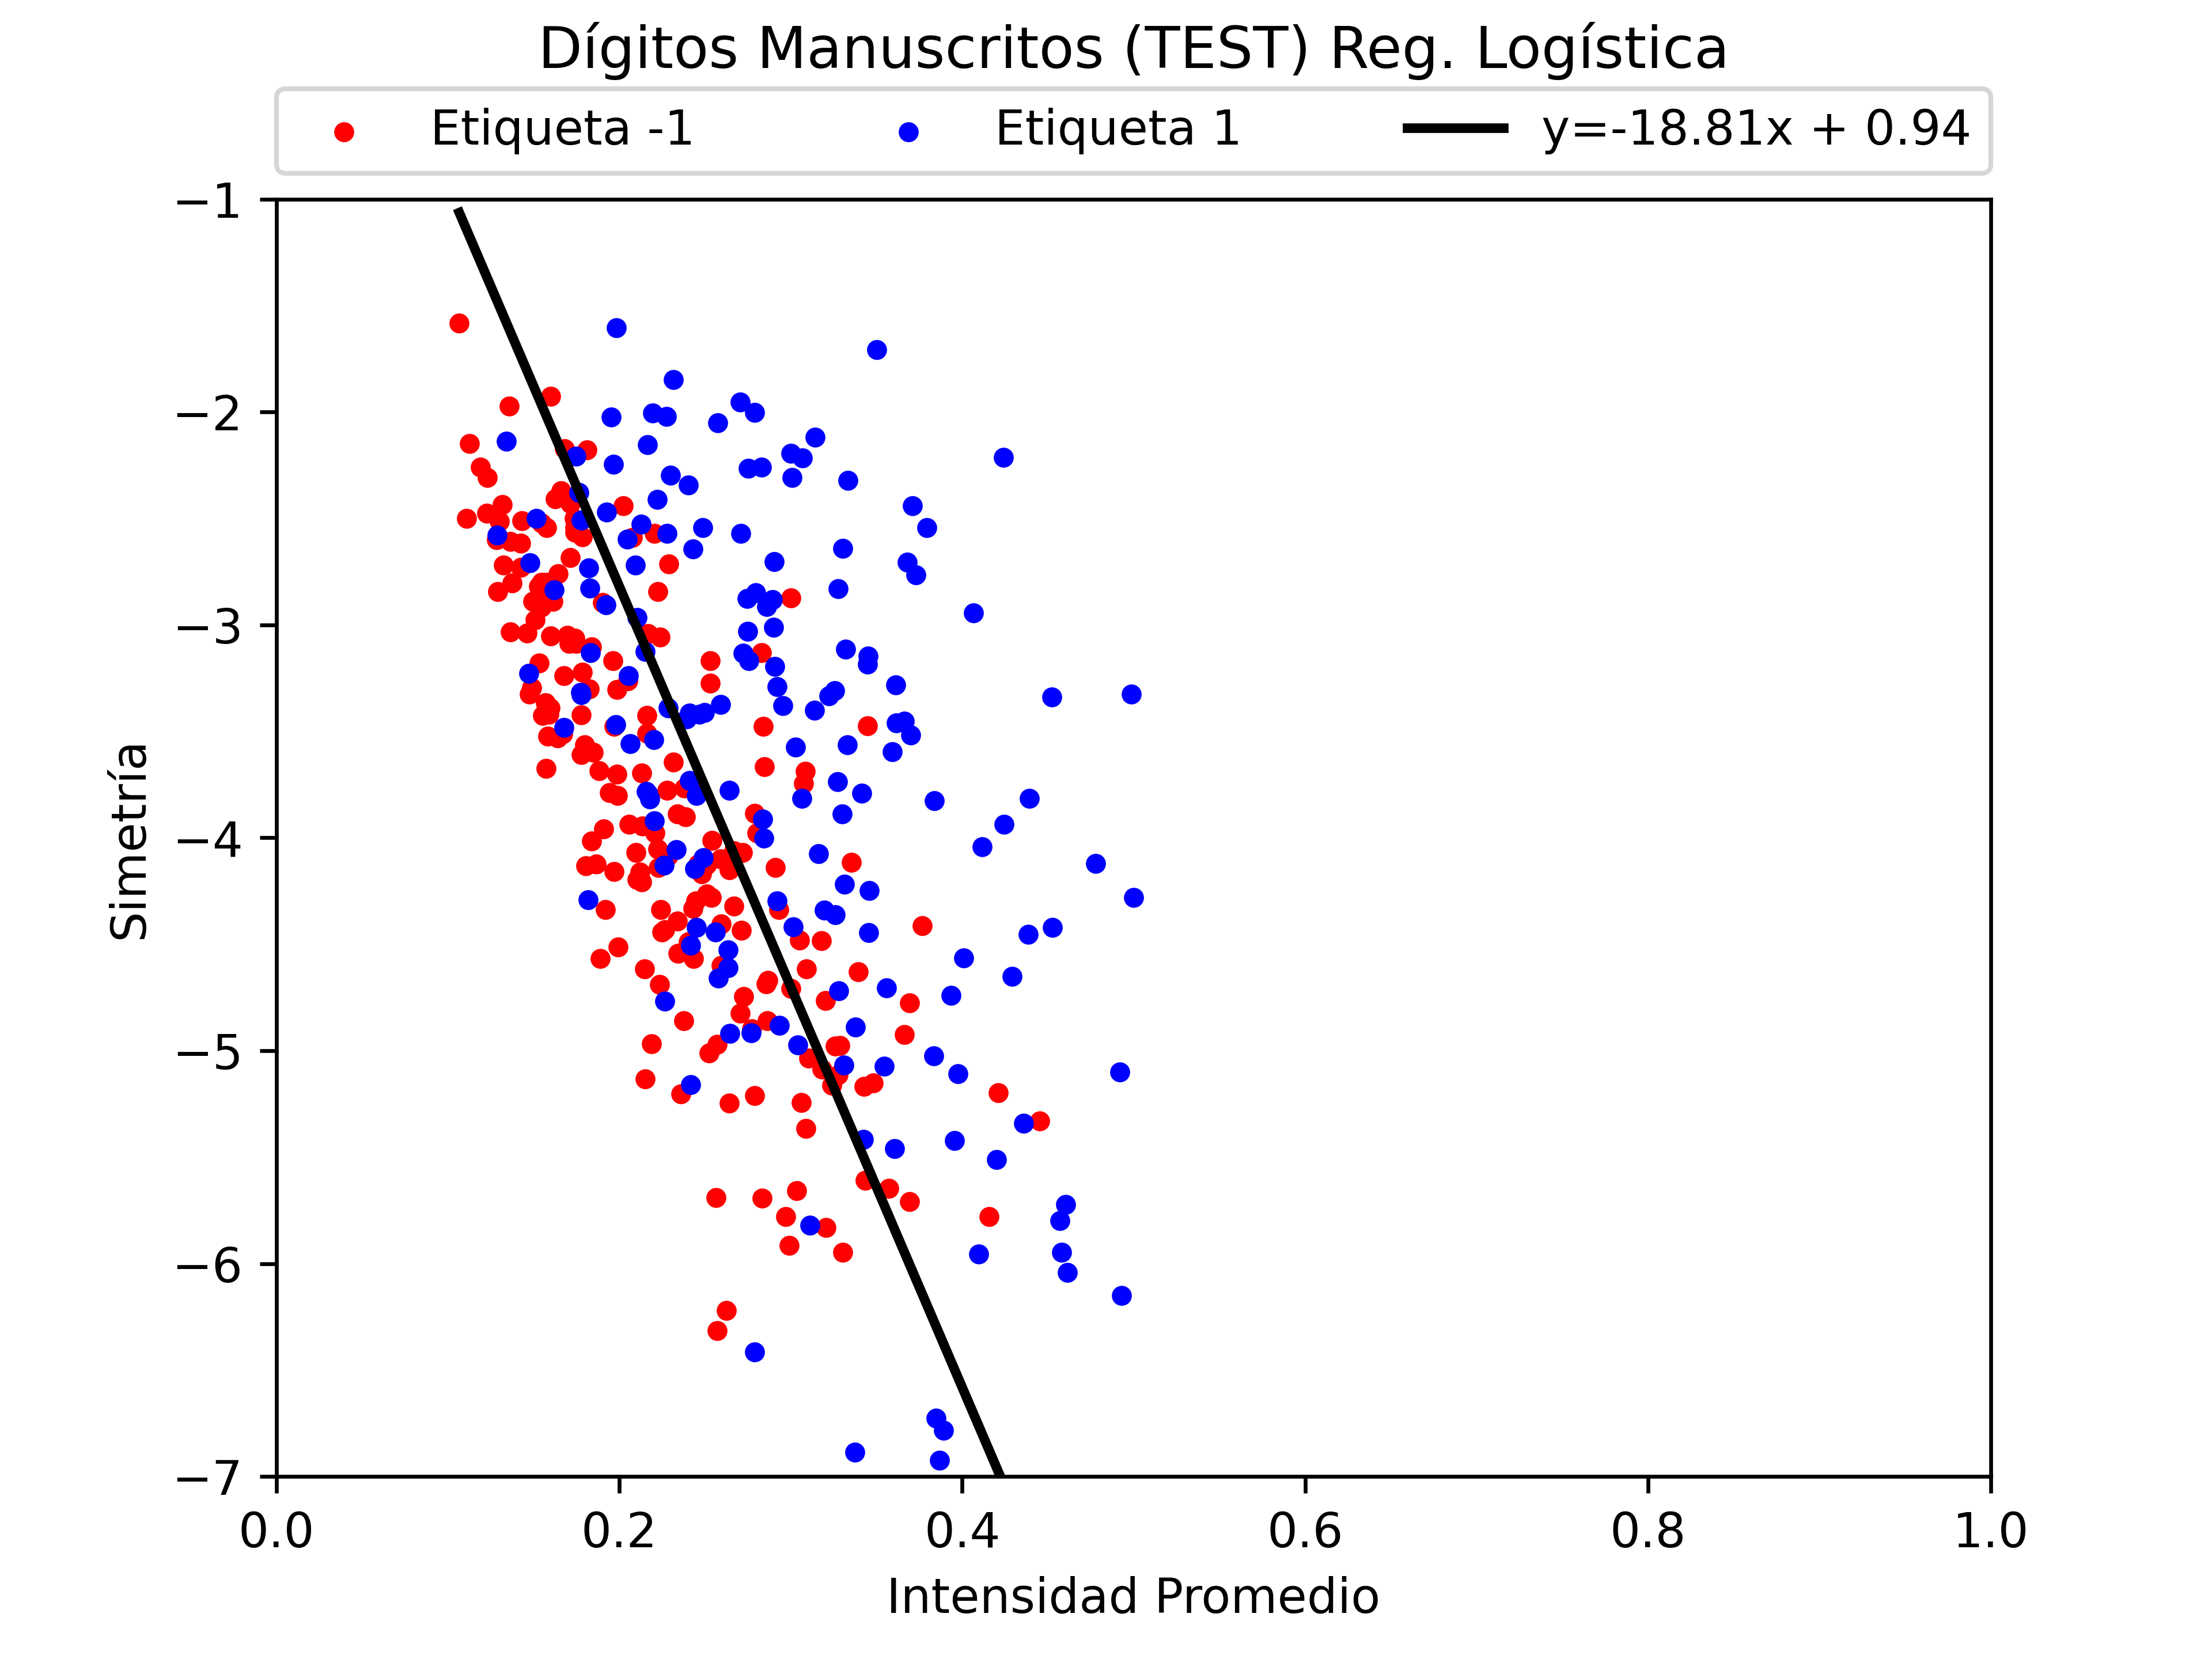
\includegraphics[width=0.9\textwidth]{Figure_26}
      \subcaption{Datos de test}
    \end{minipage}
    \label{fig:dummy67}
\end{figure}


\begin{figure}[H]
    \caption{PLA-POCKET inicializado con $w_{lin}$ \medskip}
    \begin{minipage}[b]{.5\linewidth}
      \centering
      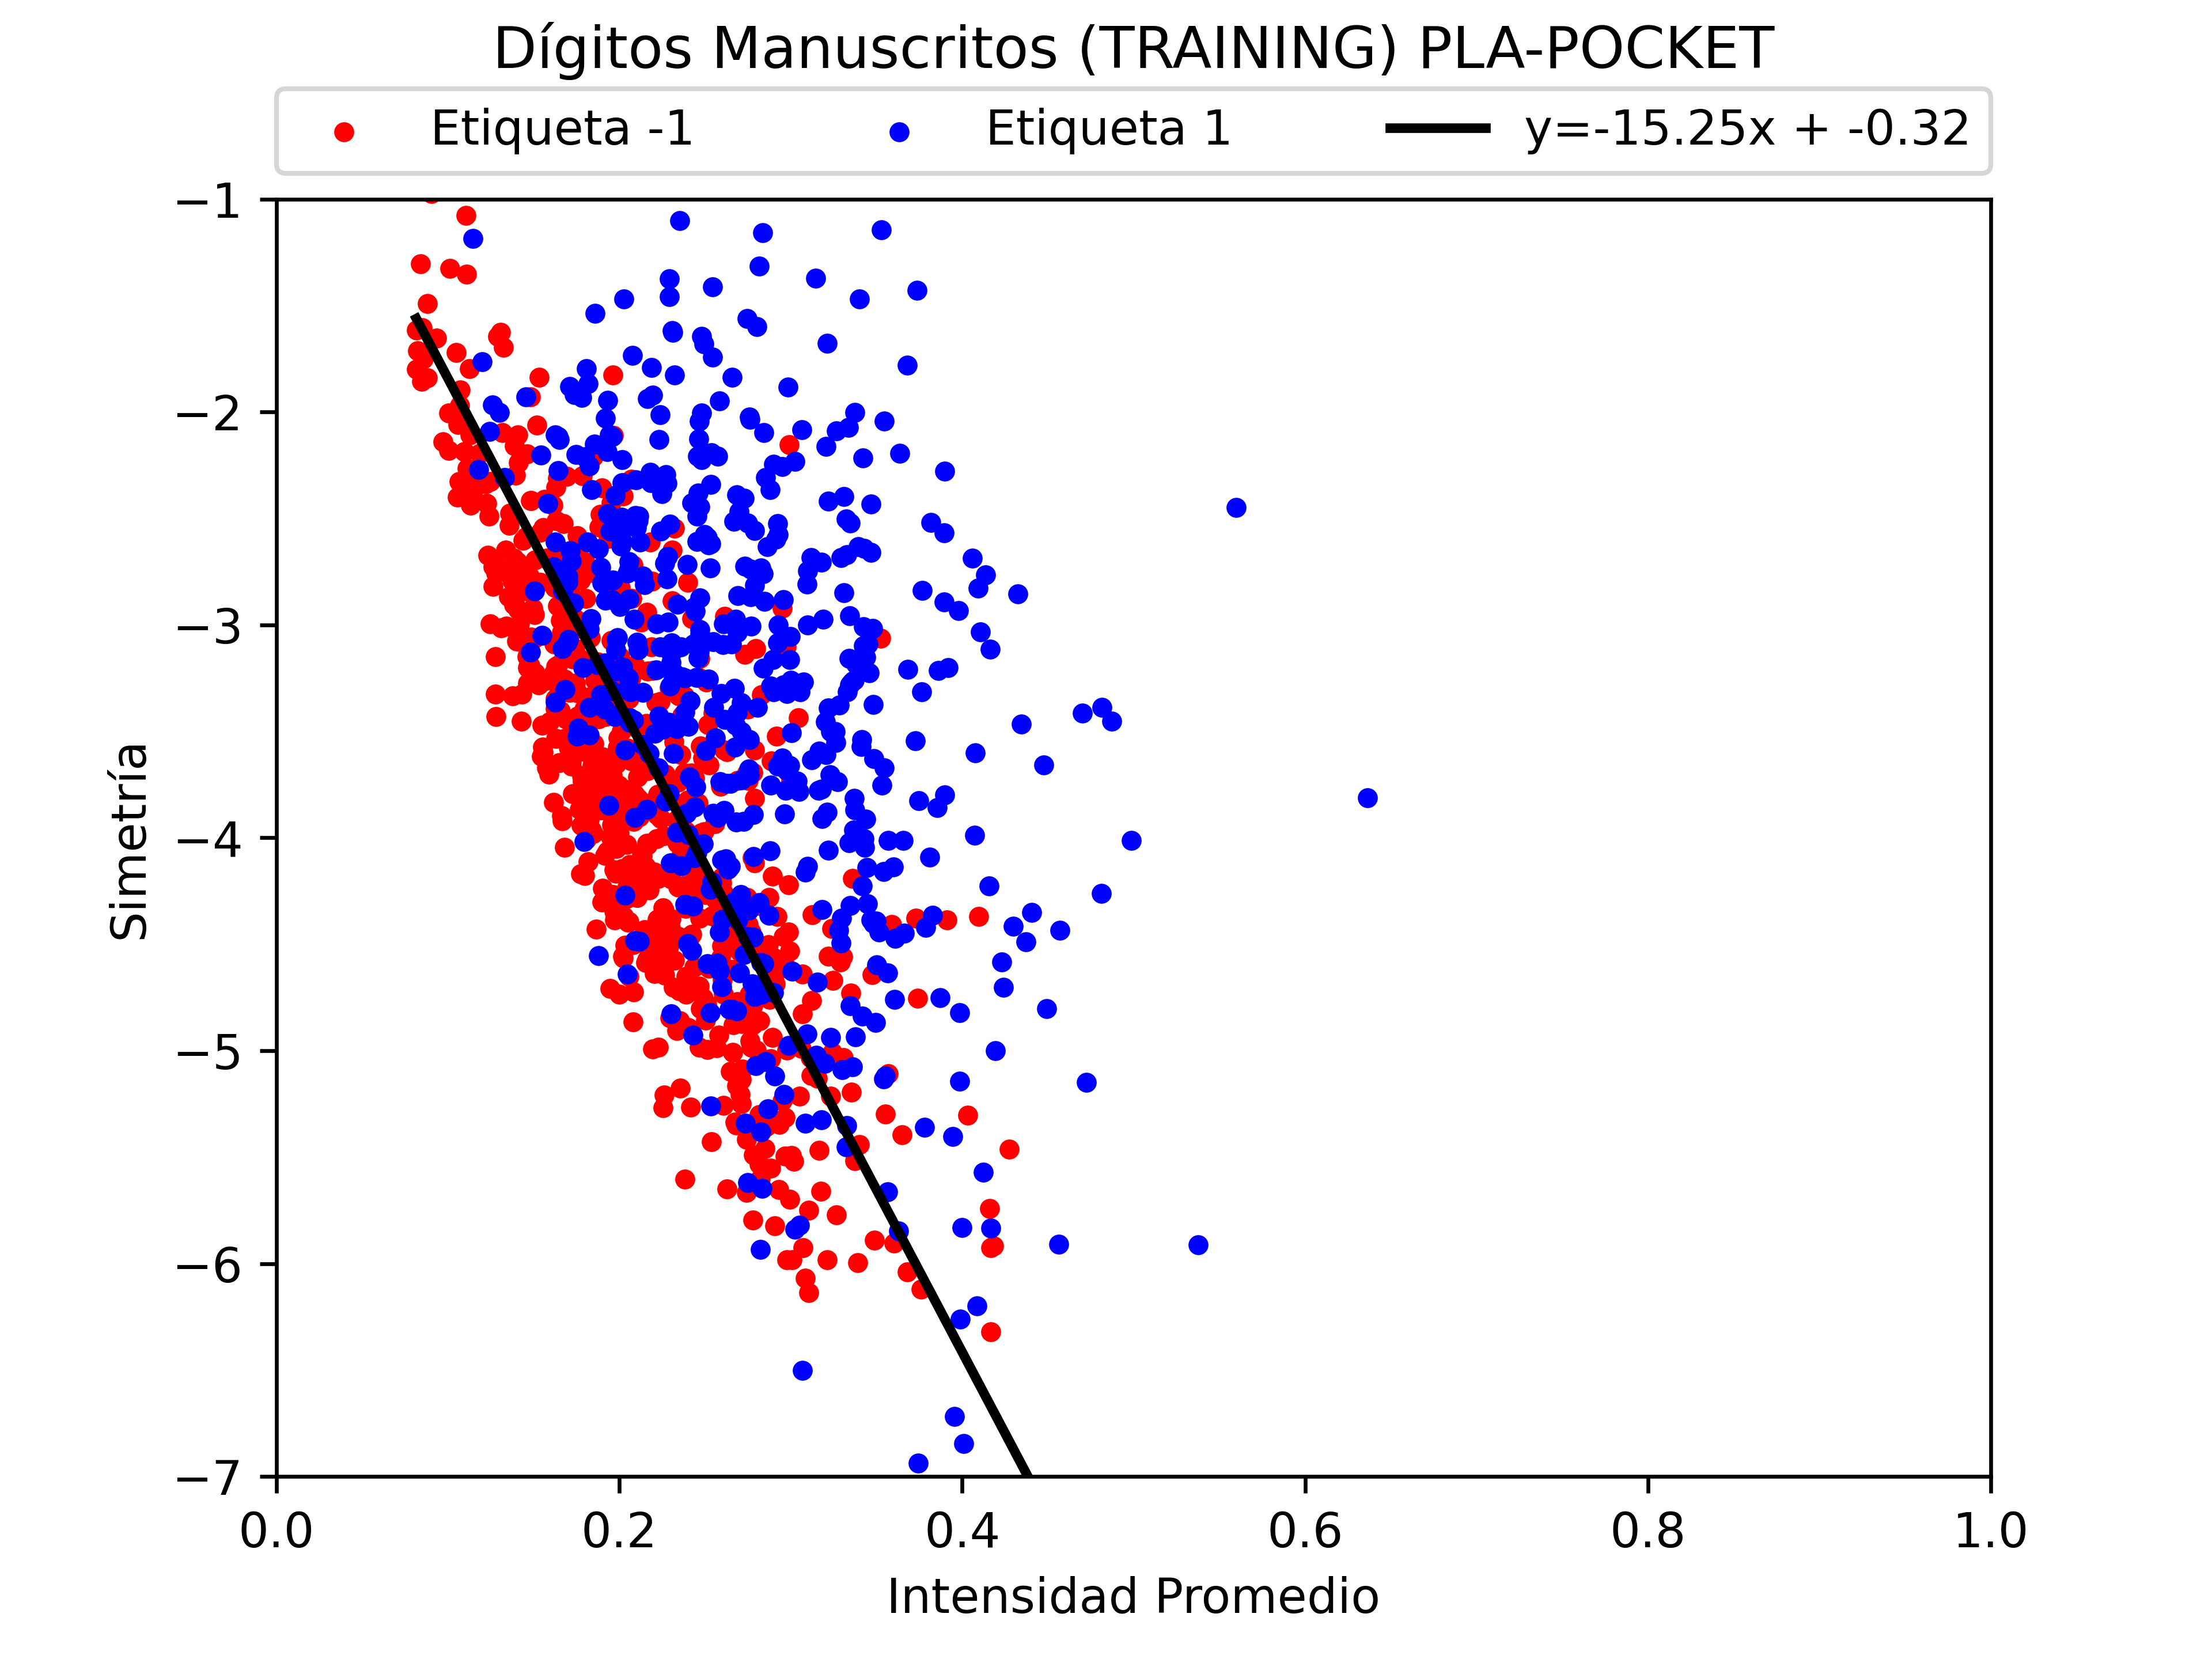
\includegraphics[width=0.9\textwidth]{Figure_27}
      \subcaption{Datos de entrenamiento} \label{subfig-5:dummy68}
    \end{minipage}
    \hfill \hfill
    \begin{minipage}[b]{.5\linewidth}
      \centering
      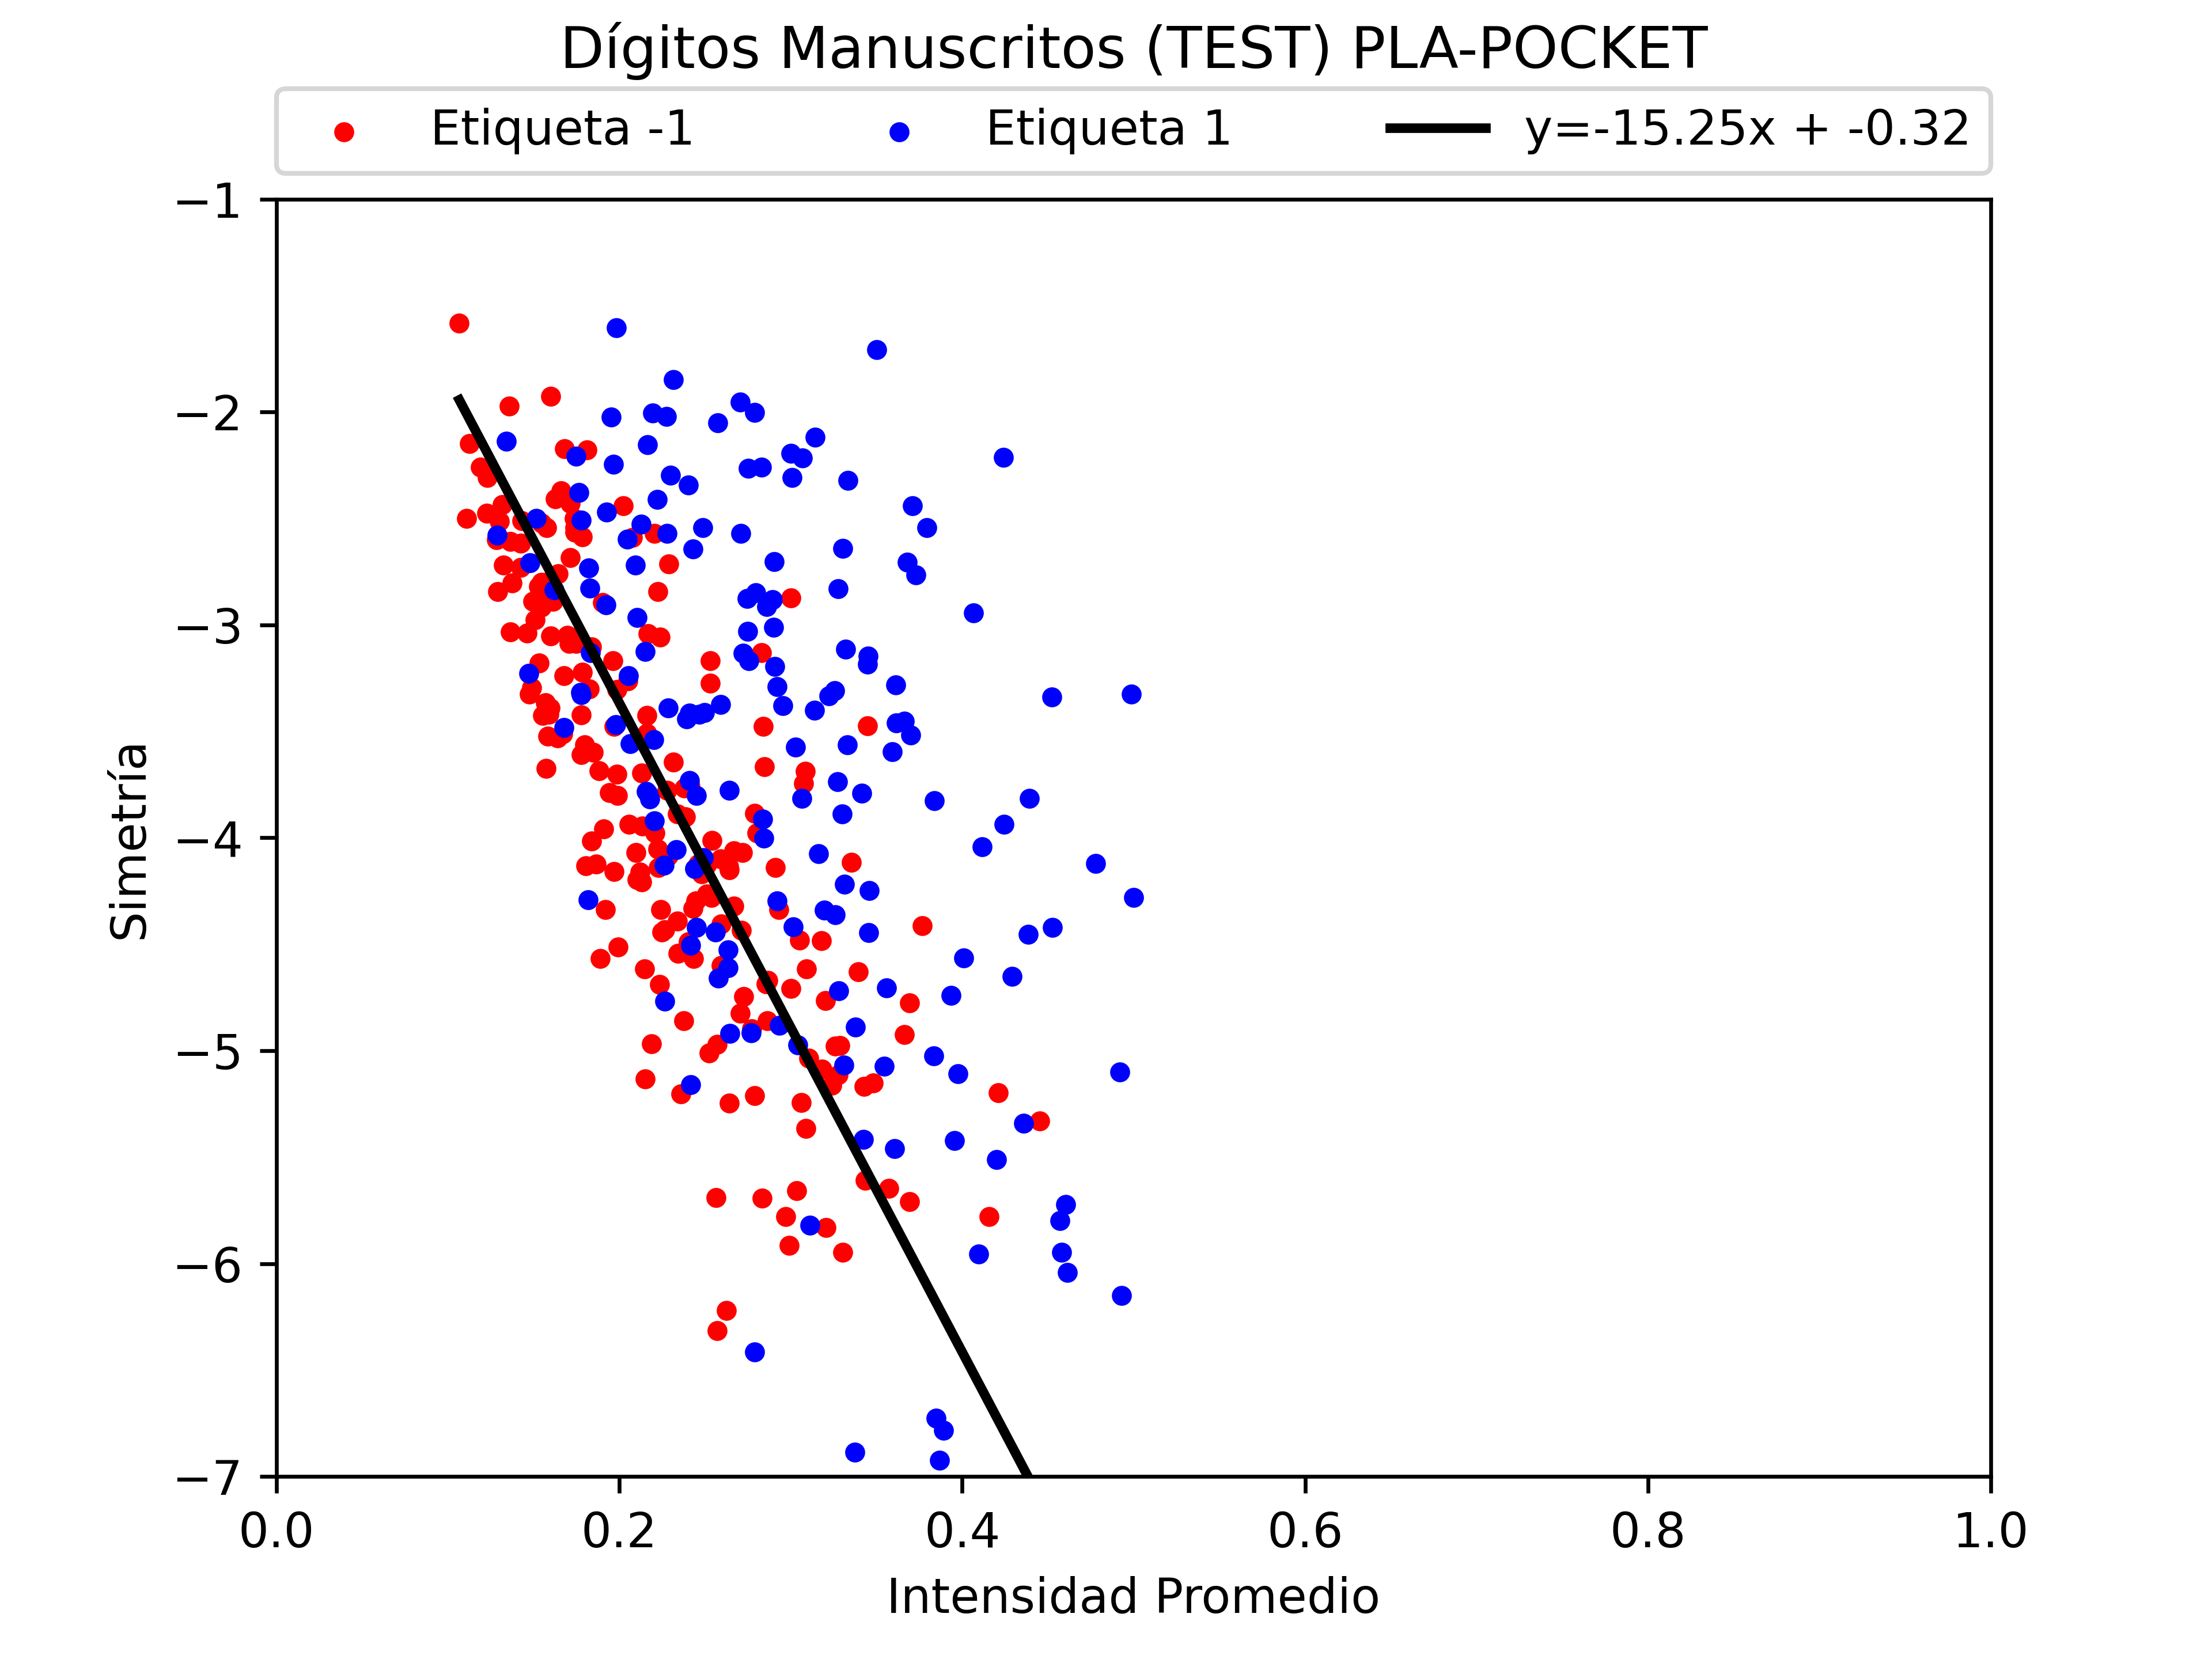
\includegraphics[width=0.9\textwidth]{Figure_28}
      \subcaption{Datos de test}
    \end{minipage}
    \label{fig:dummy68}
\end{figure}

\begin{table}[H]
    \centering
    \begin{tabular}{llllll} \toprule
        Algoritmo & $E_{in}$ & $E_{test}$ & $E_{in}^{clas}$ (\%) & $E_{test}^{clas}$ (\%) & Iteraciones \\ \midrule
        PLA & $0.252$ & $0.251$ & $25.2 \%$ & $25.1 \%$ & $1000$ \\
        RL & $0.465$ & $0.531$ & $22.2 \%$ & $26.0 \%$ & $557$ \\
        PLA-POCKET & $0.246$ & $0.322$ & $24.6 \%$ & $32.2 \%$ & $2$ \\ \bottomrule
    \end{tabular}
    \caption{Comparación de modelos lineales iterativos inicializados con $w_{lin}$}
\end{table}

En efecto, \textbf{observamos mejora en los resultados de PLA inicializado con $w_{lin}$}.
En este caso se clasifica correctamente al ($75\%$) frente al ($70\%$)
de precisión obtenido fuera de la muestra con vector inicial nulo.
Sin embargo, el error out of sample aumenta ligeramente en Regresión Logística y
PLA-POCKET con esta inicialización ($w_{lin}$) frente al vector nulo.

\subsection{Obtener cotas sobre el verdadero valor de $E_{out}$ para los 4 métodos}

\textbf{Calcúlense dos cotas: una basada en $E_{in}$ y otra basada en $E_{test}$.}
\textbf{Usar una tolerancia $\delta=0.05$.}
\textbf{¿Que cota es mejor? Justifique la respuesta.}

\subsubsection{Cota de Vapnik-Chervonenkis}

Recordamos que para $\delta > 0$, obtenemos cota de $E_{out}$ proporcionada por la expresión:

\begin{equation}
E_{out}(g) \leq E_{in} + \sqrt{\frac{8}{N}\log{\left( \frac{4 [(2N)^{d_{VC}} + 1]}{\delta} \right)}}
\end{equation}

con probabilidad $1 - \delta$ siendo $d_{VC}$ la dimensión de Vapnik-Chervonenkis del modelo y
$N$ el tamaño de $\mathcal{D}_{test}$. 

Para los 4 problemas de clasificación descritos en el primer apartado, $d_{VC} = 3$ 
de acuerdo al conjunto de hipótesis $\mathcal{H}$ y el tamaño de la muestra
de test de clasificación de dígitos es $N = 366$. Tomando $\delta = 0.05$, obtenemos

\begin{itemize}
  \item Pseudoinversa: $E_{out} \leq 0.9548$
  \item PLA ($w_{lin}$): $E_{out} \leq 0.9788$
  \item RL: $E_{out} \leq 0.9468$
  \item PLA-POCKET: $E_{out} \leq 0.9908$
\end{itemize}

lo cual no aporta gran información (entre $1\%$ y $5.4\%$ de precisión garantizada).

\subsubsection{Desigualdad de Hoeffding}

Para $\delta > 0$,

\begin{equation}
E_{out}(g) \leq E_{in}(g) + \sqrt{\frac{1}{2N}\log{\left( \frac{2 |\mathcal{H}|}{\delta} \right) }}
\end{equation}

con probabilidad $1 - \delta$. Siendo $N$ el tamaño de $\mathcal{D}_{test}$ y
$|\mathcal{H}|$ el tamaño del conjunto de hipótesis. Podemos calcular la cota a partir
de $E_{test}$ (en lugar de $E_{in}$) teniendo en cuenta que esta se verifica
para $g$ prefijado. Así $|\mathcal{H}| = 1$ y obtenemos:

\begin{itemize}
  \item Pseudoinversa: $E_{out} \leq 0.3220$
  \item PLA ($w_{lin}$): $E_{out} \leq 0.3720$
  \item RL: $E_{out} \leq E_{in} \leq 0.3220$
  \item PLA-POCKET: $E_{out} \leq 0.3520$
\end{itemize}

Concluimos por tanto, que las cotas obtenidas a partir de la desigualdad de
Hoeffding mediante $E_{test}$ son mejores que las de la dimensión VC a pesar de
ser $E_{test}$ superior a $E_{in}$. Estas cotas nos ofrecen un porcentaje de precisión 
mínimo del $68\%$ fuera de la muestra.